\chapter{Statistical Machine Translation}
\label{chap:smt}

% TODOFINAL fix vertical space after "even if one strives"
% TODOFINAL define oracles and how to compute them
% TODOFINAL talk about cmert/lmert/pro in all exps
% TODOFINAL grep for paragraph and replace by sub or subsubsection where appropriate
% TODOFINAL if time, add more hiero rule types, e.g. oov, deletions, etc.
% TODONEVER if time, expand the hiero rule extraction section with the actual implementation where holes are poled
% TODOFINAL review all equations and make sure preceded by colon rather than period.
% TODOSUBMIT rule filtering
% TODOFINAL grep for mbox and replace by text
% TODOFINAL grep for | and replace by \mid
% TODOFINAL grep footnote and replace by citation when appropriate
% TODOSUBMIT grep for ?? in pdf
% TODOFINAL check space after argmax
% TODOFINAL (done ?) ask Bill if MTTK and/or GIZA can be used for word based decoding
% TODOFINAL check word alignment vs. word-alignment
% TODOFINAL check notations with \hat: bold inside or outside the hat
% TODOFINAL grep all occurrences of start and end of sentence and use texttt
% TODOFINAL (done ?) remove the clearpage linebreaks newpages, etc.
% TODOFINAL review all source to target target to source and add hyphens
% TODOFINAL review all itemize and use consistent punctuation
% TODOFINAL add urls to thesis.bib where possible
% TODOSUBMIT (done !) grep for \cite and correct into \citet or \citep
% TODOFINAL review all transitions between sections
% TODOFINAL check title capitalization
% TODOFINAL review and expand all captions
% TODOFINAL check where sentence pair defined
% TODOFINAL check where parallel sentence, parallel corpus defined
% TODOFINAL review proper use of em dashes
% TODOFINAL check use of hierarchical phrase-based and replace with synchr gram where appropriate
% TODOFINAL check acronym MT and SMT
% TODOFINAL grep for source channel and put a hyphen
% TODOSUBMIT (done !) (remove "and colleagues")
% TODOFINAL or TODONEVER add some related work for reparameterization of model 2 and maybe discriminative alignment ?
% TODOFINAL remove vertical bar for conditional proba
% TODOFINAL replace \ by \, in multiplications
% TODOFINAL replace all {\em
% TODOFINAL remove all \bf and \it and \bfseries and \itshape
% TODOFINAL replace all refs by autoref
% TODOFINAL put a tilda before all citep
% TODOFINAL grep for trailing spaces
% TODOFINAL (done ?) add a note in the extraction from posterior chapter that we use word-to-word HMM phrase posteriors as opposed to word-to-phrase HMM phrase posteriors
% TODOFINAL (done ?) source channel or noisy channel model ?
% TODOFINAL (done ?) Bill quick question: in MTTK f2e directory, what direction is it ?
% TODOFINAL for phrase pair extraction, cite also IEEE paper, not just Yonggang thesis
% TODOFINAL (done) : papers to read: chen and goodman, yonggang IEEE, koehn's book
% TODOFINAL see alternative presentation of rule extraction in one my reading group presentations
% TODOFINAL (done !) replace all refs by autoref
% TODOFINAL replace all HMMs by mbox{HMM}
% TODOFINAL remove all mbox and replace by text
% TODOFINAL maybe cite Yee Whye Teh's 2006 paper for lm
% TODOFINAL (done) soften down claim that koehn et al is wrong in extraction from posteriors (which contradicts etc.)
% TODOFINAL (done) maybe include alignment template paper
% TODOFINAL read papers by Papineni et al 1997, Papineni et al 1998
% TODOFINAL (done) check instance of noisy channel and source channel
% TODONEVER maybe include mention of Berger et al. 1994 The Candide System
% TODOFINAL look at this paper by Venugopal et al 2003: Effective Phrase Translation Extraction from Alignment Models
% TODOFINAL look at this paper: Papineni, Roukos, and Ward (1997, 1998)
% TODOFINAL look at this paper: Comparing and Integrating Alignment Template and Standard Phrase-Based Statistical Machine Translation
% TODOFINAL look at Knight 1999 that MT search is NP-complete
% TODOFINAL learn about A* search
% TODOFINAL learn about (admissible) heuristics used in phrase-based MT
% TODOFINAL review Zens et al 2002 KI 2002
% TODOFINAL maybe look at ngram translation models
% TODOFINAL (done ?) note on how hiero models reordering directly but still can be improved a usual lexicalized reordering model
% TODOFINAL comment on hypothesis recombination and how a hyp may be lost for rescoring
% TODOFINAL maybe look at Tillmann et al 1997 for stack decoding
% TODOFINAL maybe look at A* search Och et al 2001
% TODOFINAL make a section with definitions
% TODOFINAL read the mathematics of SMT bordel de merde
% TODOFINAL grep for hyphen (phrase-based etc.)
% TODOFINAL harmonize notation \bm{f} vs. f_1^J
% TODOFINAL (done) grep for cite grep -v citep or citet
% TODOSUBMIT (done) grep for noindent
% TODOFINAL grep for {\em}, grep for {\bf}
% TODOFINAL grep for mbox
% TODOFINAL (done) grep for linebreak


% This is a background chapter on SMT with emphasis on the parts
% that will be extended further for research.

%1st year report:
%-- definition hiero grammar
%-- rule patterns
%-- generative model, log linear model
%-- features
%-- metrics
%-- mert
%-- language modelling
%-- word alignment: hmm , ctext hmm, w2p hmm, symmetrisation
%-- rule extraction
%-- decoding with wfst
%-- rescoring

%currently:
%-- generative model
%-- word alignment: hmm, w2p hmm, symmetrisation
%-- language modelling
%-- phrase-based translation
%-- mert
%-- rescoring

%missing:
%-- mapreduce

% TODOFINAL refs to background in other chapters:
%-- rule extraction alignment constraints
%-- wphmm
%-- lexical feature formula
%-- patterns and pattern filtering
%-- HiFST
%-- standard hiero grammar (patterns, etc.)
%-- mapreduce
%-- extraction constraints (retrieval and extraction)
%-- notation in background harmonized with the rest of chapters
%-- filters for grammar retrieval

%original source channel formulation OK
%word alignment OK
%newer log-linear formulation OK
%phrase-based translation OK
%hierarchical phrase-based translation OK
%features OK
%language modelling: one of the features OK
%optimization: metrics, mert OK
%hifst OK
%rescoring OK

%missing: mapreduce, phrase based translation

%\section{Overview}

% This should be an overview of the translation pipeline.
% TODOFINAL TODONEVER ? Maybe move it later as a summary and explanation of how things
% are done in practice

Statistical Machine Translation (SMT)~\citep{brown-dellapietra-dellapietra-mercer-1993,lopez:2008:ACMComputingSurveys,koehn:2010:book}
has become the dominant approach to machine translation, as increasing
amounts of data and computing power have become available.
In the SMT paradigm, given a sentence in a source language,
conceptually all
possible sentences in a target language are assigned a probability, a
score, or a cost and the best translation is picked according to a certain
decision criterion that relates to these probabilities, scores or costs.
The research challenge is to develop models that assign scores that
reflect human judgments of translation quality.

% TODOFINAL TODONEVER ? add some blabla paragraph

In this chapter, we first review the historical background of SMT in
\autoref{sec:historicalBackground}.
We then present the original source-channel model for SMT
in \autoref{sec:sourceChannelModel}.
Word alignment models, which we review in
\autoref{sec:StatisticalMachineTranslationWordAlignment},
were introduced within the framework of the source-channel
model. The original source-channel model was extended into the log-linear
model, presented in \autoref{sec:loglinearModel}.
The field of SMT shifted from word-based models to phrase-based
models, introduced in \autoref{sec:phraseBasedTranslation}, while
retaining word-based models in their first formulation as a preliminary step.
Phrase-based translation was extended into hierarchical
phrase-based translation, which we review in
\autoref{sec:hierarchicalPhraseBasedTranslation}.
% TODOFINAL (done ?) put this somewhere else, e.g. in motivation section of hierarchical phrase based mt
%Hierarchical phrase-based translation model
%``gappy'' phrases and reordering
%with a probabilistic synchronous context-free grammar.
We then
examine various features employed in state-of-the-art decoders in
\autoref{sec:features}. The target language model, which
is one of the most important features in translation, is explored in
more detail in \autoref{sec:languageModelling}. In
\autoref{sec:optimization}, we review optimization techniques that
are employed in order to tune the decoder parameters. We finally present
how finite state transducers can be used in decoding
in \autoref{sec:hifst}. Various rescoring
procedures are reviewed in \autoref{sec:rescoring}.

% TODO MapReduce !!!!!!!!!!!!!!!!!!!!!!

\section{Historical Background}
\label{sec:historicalBackground}

%\begin{itemize}
%  \item warren weaver and the Translation report
%  \item development of rule based systems
%  \item development of word based systems + source channel model
%  \item development of phrase based systems + discr model
%  \item development of syntactic systems
%  \item neural networks ????
%\end{itemize}

%warren weaver
%historical survey: From First Conception to First Demonstration: the Nascent Years of Machine Translation, 1947–1954. A Chronology
%emphasize that the initial idea at a time when the idea is possible to implement dates from warren weaver. before that, just speculation since computers did not exist.
%talk about resurgence in mt of interlingua methods (tomas mikolov and word2vec software)
%mention quicksort as application of MT ?
%warren weaver Translation report: word 2 word translation not good. multiple meaning solution: look at context
%translation and cryptography a book written in Chinese is simply a book written in English which was coded into the the "Chinese code".
%translate with a certain confidence.
%language invariants: machine translation pyramid, interlingua, shout from building to building or go through the tunnel

In this section, we present a brief historical background of \emph{statistical}
machine translation. A more comprehensive account of the history
of machine translation in general can be found
elsewhere~\citep{hutchins:1997:MT,hutchins:2000:MT}.

Warren Weaver can be considered the father of modern SMT.
At a time when the first computers were being developed, he
examined their potential application to the problem of machine
translation. In his memorandum~\citep{weaver:1955:Translation}, he
addressed the problem of multiple meanings of a source word
by considering the context of that source word, which heralds
phrase based translation techniques and the use of context
in machine translation. He was also
the first to frame machine translation as a source-channel
model by considering that a sentence in a foreign language
is some form of code that needs to be broken, in analogy
to the field of cryptography. Finally, he also emphasized the
statistical aspect of machine translation. However, he also
predicted that the most successful approaches to machine
translation would take advantage of language invariants by
using an intermediate language representation in the translation
process. Even though state-of-the-art statistical translation systems do not
use this kind of approach, we do notice a resurgence in intermediate
language representation techniques~\citep{mikolov-le-sutskever:2013:arxiv}.

The first successful implementations of Warren Weaver's ideas
were carried out by IBM in the 1990s. The source-channel
model together with a series of word alignment models were introduced
by~\citet{brown-dellapietra-dellapietra-mercer-1993} while
\citet{berger-dellapietra-dellapietra:1996:CL} addressed the problem
of multiple meanings using context in a maximum entropy framework.
Word-based models were extended into different variants
of phrase-based models in 1999 and at the
beginning of the
century~\citep{och-tillmann-ney:1999:EMNLP,koehn-och-marcu:2003:NAACL,och-ney:2004:CL}
and later on into synchronous context-free grammar
models~\citep{chiang:2005:ACL,chiang:2007:CL}.

\section{Source-Channel Model}
\label{sec:sourceChannelModel}
% TODOFINAL (done) check whether we say noisy channel or source channel model
% TODOFINAL (done ?) normalize SMT
%brown et al series of papers directly inspired by warren weaver

%additional papers:
%brown et al 90: a statistical approach to machine translation


%notes for: a statistical approach to language translation
%glossary creation
%in the intro, phrase-based translation is basically described !!! partition source text into set of fixed locution (~ phrase), use glossary + contextual info to translate
%the phrases, arrange words in the target !!!!!!!!!!!!!!!!!!!!!!!!!!
%find word pairs using maximum mutual information criterion

Statistical machine translation was originally framed as a source-channel
model~\citep{shannon:1948:BellSystemTechnicalJournal,brown-cocke-dellapietra-dellapietra-jelinek-lafferty-mercer-roossin:1990:CL,brown-dellapietra-dellapietra-mercer-1993}.
Given a
foreign sentence $\bm{f}$, we want to find the original English sentence
$\bm{e}$ that went through a noisy channel and produced $\bm{f}$. Note that in
the source-channel model notation, what we would like to
recover---the English sentence---is
called the \emph{source} while what is observed---the foreign sentence---is
called the \emph{target}. A source-channel model assigns probabilities
from source (English) to target (foreign) but in translation, the model
is used to infer the source that was most likely to have generated
the target.

We do not use this convention here and call the
\emph{source} what we are translating from and the \emph{target} what we are
translating into. This convention is frequently
adopted~\citep{och-tillmann-ney:1999:EMNLP,och-ney:2002:ACL,och-ney:2004:CL}
in SMT,
and more so since SMT has been framed as a log-linear
model (see \autoref{sec:loglinearModel}). We use the
decision rule in \autoref{eq:noisy}, which minimises the risk under
a zero-one loss function (see \autoref{sec:lmbr}):
%
\begin{align}
  \bm{\hat{e}} &= \argmax_{\bm{e}} p(\bm{e} \mid \bm{f}) \nonumber \\
  \bm{\hat{e}} &= \argmax_{\bm{e}} \frac{p(\bm{f} \mid \bm{e}) \, p(\bm{e})}{p(\bm{f})} \mbox{ (Bayes' rule)} \nonumber \\
  \bm{\hat{e}} &= \argmax_{\bm{e}} p(\bm{f} \mid \bm{e}) \, p(\bm{e}) \label{eq:noisy}
\end{align}
%
$\bm{\hat{e}}$ is the hypothesis to be selected.
$p(\bm{f} \mid \bm{e})$ is called the \emph{translation model} while
$p(\bm{e})$ is called the (target) \emph{language model}.

The translation model and the language model are estimated separately
for practical reasons: the amount of parallel data used to train the translation
model is in general orders of magnitude smaller than the amount of monolingual
data used to train the language model. Another justification is that
using two separate models makes the translation process modular: improving
the translation model may help improve \emph{adequacy}, i.e.\ how well the meaning
of the source text is preserved in the translated text, while improving
the language model may help improve \emph{fluency}, i.e.\ how well-formed the
translation is. It is therefore considered
preferable to train both a translation model and a language model.
In these models, parallel sentence pairs and target sentences are
not used directly as parameters because of an obvious sparsity
problem. Parallel sentence pairs are further broken down using
word-based models (see \autoref{sec:StatisticalMachineTranslationWordAlignment}),
phrase-based models (see \autoref{sec:phraseBasedTranslation})
and hierarchical phrase-based models
(see \autoref{sec:hierarchicalPhraseBasedTranslation}). For language
modelling, sentences are broken down into windows of consecutive
words using $n$-gram language models (see \autoref{sec:languageModelling}).
We will see in the next section how to decompose
the translation model using word alignment, which is
introduced as a latent variable into the source-channel model.

\section{Word Alignment}
\label{sec:StatisticalMachineTranslationWordAlignment}

In the previous section, we have briefly described the source-channel model, which
describes the translation process. This model cannot be used directly in
practice as it has too many parameters, namely all imaginable
sentence pairs and target sentences. In order to address this issue,
the \emph{alignment} between source words and target words will be
introduced as a latent variable in the source channel model.

Given a sentence pair $(\bm{f}, \bm{e})$ with source sentence
length $J = |\bm{f}|$ and target sentence
length $I = |\bm{e}|$, a \emph{word alignment} $\bm{a}$
for this sentence pair is a mapping between the source and target
words. In other words, $\bm{a}$ is a subset of the cross product
of the set of source words and their positions and the set of target
words and their positions, as defined in \autoref{eq:alignmentSetDefinition}:
%
\begin{equation}
  \bm{a} \subset \{((f_j, j), (e_i, i)), (j, i) \in [1, J] \times [1, I]\}
  \label{eq:alignmentSetDefinition}
\end{equation}
%
When the context of which sentence pair $(\bm{f}, \bm{e})$ is
being word-aligned is obvious, we may simply consider source word positions
and target word positions. In that case, $\bm{a}$ is simply defined
as a subset (source position, target position), in
\autoref{eq:alignmentSetDefinitionSimpler}:
%
\begin{equation}
  \bm{a} \subset [1, J] \times [1, I]
  \label{eq:alignmentSetDefinitionSimpler}
\end{equation}
%
Each element of $\bm{a}$ is called an \emph{alignment link}.
Alignment links between source and target words
correspond to semantic or syntactic equivalences shared by these words in the
source and target language and in a particular
sentence pair. Alignments can present many-to-one and one-to-many
mappings as well as reordering as highlighted by crossing links. An example
of word alignment is
shown in \autoref{fig:examplealign}.
% TODONEVER maybe add circles around the words
%
\begin{figure}
  \begin{center}
  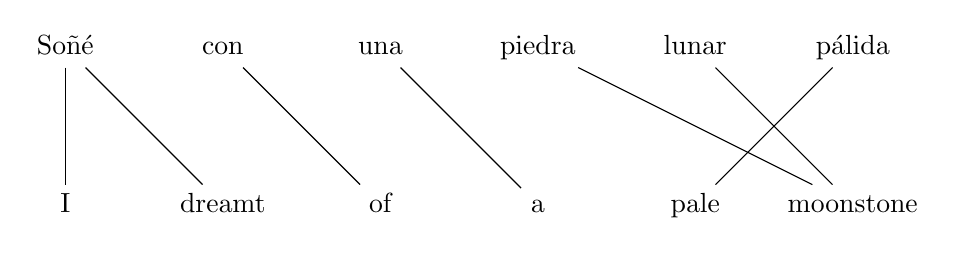
\begin{tikzpicture} [node distance = 2cm, text height=1.5ex, text depth=.25ex]
    % place nodes
    \node (Sone) {Soñé};
    \node [right of = Sone] (con) {con};
    \node [right of = con] (una) {una};
    \node [right of = una] (piedra) {piedra};
    \node [right of = piedra] (lunar) {lunar};
    \node [right of = lunar] (palida) {pálida};
    \node [below of = Sone] (I) {I};
    \node [right of = I] (dreamt) {dreamt};
    \node [right of = dreamt] (of) {of};
    \node [right of = of] (a) {a};
    \node [right of = a] (pale) {pale};
    \node [right of = pale] (moonstone) {moonstone};
    % draw edges
    \draw (Sone) -- (I);
    \draw (Sone) -- (dreamt);
    \draw (con) -- (of);
    \draw (una) -- (a);
    \draw (piedra) -- (moonstone);
    \draw (lunar) -- (moonstone);
    \draw (palida) -- (pale);
  \end{tikzpicture}
  \end{center}
  \caption{Example of word alignment $\bm{a}$ for a Spanish-English sentence pair.
    $\bm{f}$ is the Spanish sentence, $\bm{e}$ is the English sentence.
    The source (Spanish)
    length $J$ is 6 as well as the target (English) length $I$. This alignment
    exhibits many-to-one mappings (\emph{I} and \emph{dreamt} align
    to \emph{Soñé}), one-to-many mappings (\emph{moonstone} aligns
    to \emph{piedra} and \emph{lunar}), as well as crossing links
    (the link \emph{pale}---\emph{pálida} crosses the
    link \emph{moonstone}---\emph{lunar}).}
  \label{fig:examplealign}
\end{figure}
%

\citet{brown-dellapietra-dellapietra-mercer-1993} introduce the
alignment $\bm{a}$ as a latent variable in the translation model
$p(\bm{f} \mid \bm{e})$, as in \autoref{eq:introduceAlignment}:
\begin{equation}
  p(\bm{f} \mid \bm{e}) = \sum_{\bm{a}} p(\bm{f}, \bm{a} \mid \bm{e})
  \label{eq:introduceAlignment}
\end{equation}
%
We abuse notation by calling $\bm{a}$ both the latent variable
and the set of alignment links, which is an instance of the latent
variable.
For mathematical convenience and in order to allow simplifications,
given a sentence pair $(\bm{f}, \bm{e})$ with source length
$J$ and target length $I$,
$\bm{a}$ is restricted to be a function from source word positions
to target word positions, as in \autoref{eq:alignmentDefinition}:
%
\begin{equation}
\begin{split}
  \bm{a} : [1, J] &\longrightarrow [0, I] \\
                j &\longmapsto a_j
\end{split}
\label{eq:alignmentDefinition}
\end{equation}
%
The target position zero is included to
model source words not aligned to any target word; these unaligned source words
are virtually aligned to a so-called \emph{null word}. Note that this definition
is not symmetric: it only allows many-to-one mappings from source to target.
Various symmetrisation strategies, presented in \autoref{sec:symmetrisationHeuristics},
have been devised to address this limitation.
Also note that we did not
take into account the null word in our initial definition of alignments
in \autoref{eq:alignmentSetDefinition} because in general, alignments
are obtained from symmetrisation heuristics
(see \autoref{sec:symmetrisationHeuristics}) where the null word
is ignored.
We can use the latent variable
$\bm{a}$ to rewrite the translation model in
\autoref{eq:generalEquationIBMModels}, with $\bm{f} = f_1^J$, $\bm{e} = e_1^I$
and $\bm{a} = a_1^J$:
%
\begin{equation}
  \begin{split}
    p(f_1^J \mid e_1^I) &= \sum_{a_1^J} p(f_1^J, a_1^J \mid e_1^I) \\
                        &= \sum_{a_1^J} \prod_{j = 1}^J p(f_j, a_j \mid f_1^{j - 1}, a_1^{j - 1}, e_1^I) \\
                        &= \sum_{a_1^J} \prod_{j = 1}^J p(f_j \mid f_1^{j - 1}, a_1^j, e_1^I) \, p(a_j \mid f_1^{j - 1}, a_1^{j - 1}, e_1^I) \\
  \end{split}
  \label{eq:generalEquationIBMModels}
\end{equation}
%
\citet{brown-dellapietra-dellapietra-mercer-1993} present a series
of five translation models of increasing complexity that parameterise the terms
$p(f_j \mid f_1^{j - 1}, a_1^j, e_1^I)$ and
$p(a_j \mid f_1^{j-1}, a_1^{j-1}, e_1^I)$.
Parameter estimation is carried out with the
expectation-maximisation algorithm~\citep{dempster-laird-rubin:1977:JRSS}.
Also based on \autoref{eq:generalEquationIBMModels}, \citet{vogel-ney-tillmann}
introduce an HMM model~\citep{rabiner:1989:IEEE} for
word alignment and \citet{deng-and-byrne:2008:ASLP}
extend the HMM model to a word-to-phrase HMM model. We describe these two models in the following
sections.
% TODONEVER should I present all IBM models ???

% TODOFINAL think about where to put this
We have described word alignment models in the context of the source-channel
model. In that context, word alignment models can be used directly for word-based
decoding.\footnote{e.g. \url{http://www.isi.edu/licensed-sw/rewrite-decoder}} % TODOFINAL (done) check whether MTTK and/or GIZA++ can also be used in decoding mode
However, nowadays, word alignment models are used as a preliminary
step in the machine translation training pipeline, namely
prior to rule extraction (see \autoref{sec:phrasextract} and
\autoref{sec:hierruleextract}). In that case,
the word alignment models are used to produce Viterbi alignments, defined
in \autoref{eq:viterbiAlignment}:
%
\begin{equation}
  %\begin{split}
    %\hat{a}_1^J &= \argmax_{a_1^J} p(a_1^J \mid f_1^J, e_1^I) \\
    \hat{a}_1^J = \argmax_{a_1^J} p(f_1^J, a_1^J \mid e_1^I)
  %\end{split}
  \label{eq:viterbiAlignment}
\end{equation}
%
One contribution of this
thesis is to use alignment posterior probabilities instead of
Viterbi alignments for rule
extraction (see \autoref{chap:extractionFromPosteriors}).

\subsection{HMM and Word-to-Phrase Alignment Models}
\label{sec:statisticalMachineTranslationHmmAlignmentModel}

% notes on Yonggang's 2008 journal paper
%in the paper notation, assuming translation is from foreign to English,
%source denotes English (target in thesis notation) and target denotes
%foreign (source in thesis notation)
%source sentence of I words s = s_1^I
%target sentence of J words t = t_1^J
%target sentence segmented into K target phrases
%target phrases: v_1^K
%each v_k generated by a single word in the source phrase
%correspondence source words target phrases: alignment a_1^K
%s_{a_k} -> v_k
%number of words in each target phrase: phi_k
%constraint: J = sum_{k=1}^K phi_k
%NULL source word
%alternative to NULL word: h_1^K hallucination sequence
%h_k = 0: NULL -> v_k; h_k = 1: s_{a_k} -> v_k
%a = (phi_1^K, a_1^K, h_1^K, K)
%p(t,a|s) = p(v_1^K, K, a_1^K, h_1^K, phi_1^K | s)


We review HMM and word-to-phrase HMM models as these models are used
in experiments throughout this thesis.
\citet{vogel-ney-tillmann} introduce an HMM alignment model
that treats target word positions as hidden states and source words as
observations. The model is written in \autoref{eq:HmmAlignmentDefinition}:
%
\begin{equation}
  p(f_1^J, a_1^J \mid e_1^I) = \prod_{j=1}^J p(a_j \mid a_{j-1},I) \, p(f_j \mid e_{a_j})
  \label{eq:HmmAlignmentDefinition}
\end{equation}
%
Word-to-phrase HMM models~\citep{deng-and-byrne:2008:ASLP} were designed to
capture interesting properties of IBM Model
4~\citep{brown-dellapietra-dellapietra-mercer-1993} in an HMM framework in order
to keep alignment and estimation procedures exact. We now present this model
in more detail, using our usual source/target convention, which is the reverse
than the one adopted in the original
publication\footnote{$\bm{s}$ in the publication corresponds to $\bm{e}$ in this thesis;
$\bm{t}$ corresponds to $\bm{f}$; $J$ corresponds to $J$; $I$ corresponds to $I$.}.
In the word-to-phrase HMM alignment model, the source sentence
$\bm{f}$ is segmented into source phrases $v_1^K$.
The alignment $\bm{a}$ is represented by a set of variables
$(\phi_1^K, a_1^K, h_1^K, K)$ where:
%
\begin{itemize}
  \item $K$ is the number of source phrases that form a segmentation of the source sentence $\bm{f}$.
  \item $a_1^K$ is the alignment from target words to source phrases.
  \item $\phi_1^K$ indicates the length of each source phrase.
  \item $h_1^K$ is a \emph{hallucination} sequence that indicates whether
    a source phrase was generated by the target null word
    or by a usual target word.
\end{itemize}
%
The general form of the model is presented in \autoref{eq:word2phraseHmmGeneral}:
%
\begin{equation}
  \begin{split}
  p(\bm{f}, \bm{a} \mid \bm{e}) = & \; p(v_1^K, K, a_1^K, h_1^K, \phi_1^K \mid \bm{e}) \\
                                = & \; p(K \mid J, \bm{e}) \times \\
                                & \; p(a_1^K, \phi_1^K, h_1^K \mid K, J, \bm{e}) \times \\
                                & \; p(v_1^K \mid a_1^K, h_1^K, \phi_1^K, K, J, \bm{e})
  \end{split}
  \label{eq:word2phraseHmmGeneral}
\end{equation}
%
We now review the modelling decisions taken for each
of the components from \autoref{eq:word2phraseHmmGeneral}.
The first component is simply modelled by:
%
\begin{equation}
  p(K \mid J, \bm{e}) = \eta^K
\end{equation}
%
where $\eta$ is a threshold that controls the number of segments in the source.
The second component is modelled using the Markov assumption:
%
\begin{align}
  p(a_1^K, \phi_1^K, h_1^K \mid K, J, \bm{e})
    &= \prod_{k = 1}^K p(a_k, h_k, \phi_k \mid a_{k - 1}, \phi_{k - 1}, h_{k - 1}, K, J, \bm{e}) \nonumber \\
    &= \prod_{k = 1}^K p(a_k \mid a_{k - 1}, h_k, I) \, d(h_k) \, n(\phi_k \mid e_{a_k})
\end{align}
%
As in the HMM word alignment model $a_k$ depends only on $a_{k - 1}$, the target
length $I$ and the binary value $h_k$. $d(h_k)$ is simply controlled by the
parameter $p_0$ by $d(0) = p_0$. $n(\phi_k \mid e_{a_k})$ is a finite distribution
on source phrase length that depends on each target word and which plays the role
of a fertility parameter.

The third component from \autoref{eq:word2phraseHmmGeneral} is defined in
\autoref{eq:word2phraseTranslation} and represents the word-to-phrase translation parameter:
%
\begin{equation}
  p(v_1^K | a_1^K, h_1^K, \phi_1^K, K, J, \bm{e}) = \prod_{k = 1}^K p(v_k \mid e_{a_k}, h_k, \phi_k)
  \label{eq:word2phraseTranslation}
\end{equation}
%
One key contribution from the word-to-phrase HMM model is to use bigram translation
probabilities to model one single phrase translation, as shown
in \autoref{eq:bigramTranslation}:
%
\begin{equation}
  p(v_k \mid e_{a_k}, h_k, \phi_k) = t_1(v_k[1] \mid h_k \cdot e_{a_k}) \prod_{j = 2}^{\phi_k} t_2(v_k[j] \mid v_k[j - 1], h_k \cdot e_{a_k})
  \label{eq:bigramTranslation}
\end{equation}
%
where $h_k \cdot e_{a_k}$ is $e_{a_k}$ if $h_k = 1$ and the null word otherwise, $t_1$ is
a word-to-word translation probability and $t_2$ is a bigram translation probability.

\autoref{fig:wordtophrase}
shows a simplified version of the generative story for an HMM word-to-phrase
alignment model: first, pick the number of source phrases $K$ according to
$P(K \mid J,I)$; then
pick a target word given the previously chosen one; finally generate the target
phrase from the source word using fertility and bigram translation probabilities.
For example, we generate the source phrase \emph{les vaches} from
the target word \emph{cows}
according to \autoref{eq:exampleBigramTranslation}:
%
\begin{equation}
  p(\text{\emph{les vaches}} \mid \text{\emph{cows}}) = p(\text{\emph{les}} \mid \text{\emph{cows}}) \, p(\text{\emph{vaches}} \mid \text{\emph{cows}}, \text{\emph{les}})
  \label{eq:exampleBigramTranslation}
\end{equation}
%
Thus bigram probabilities take into account the context of the target word to
some extent.
%
%\begin{figure}
%  \begin{center}
%    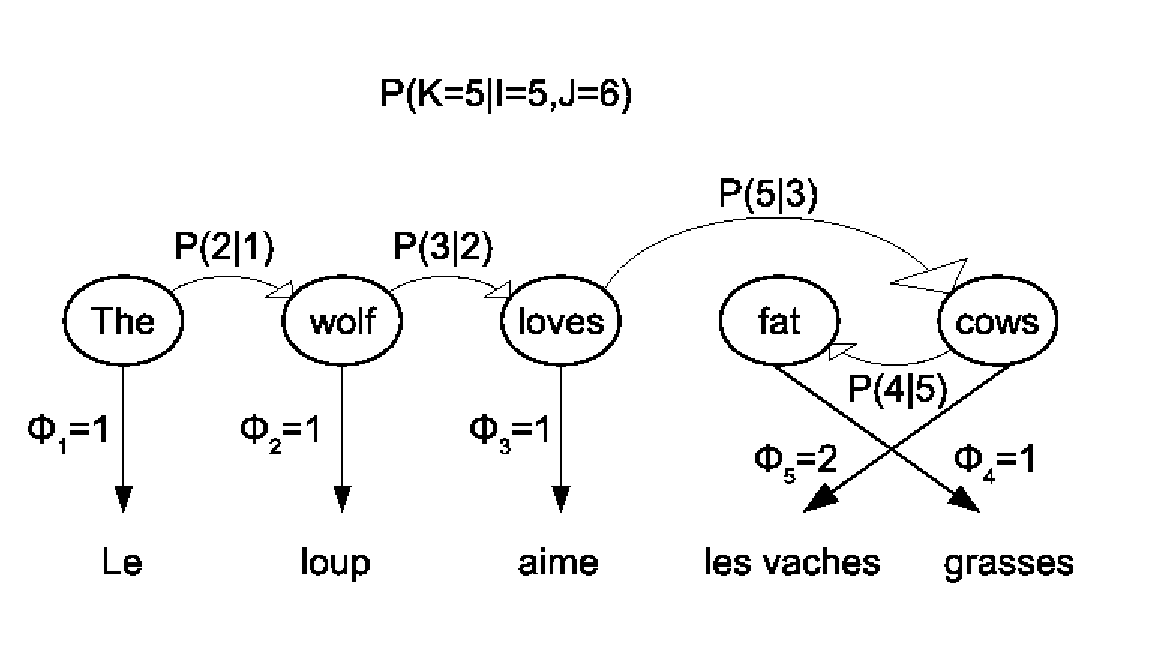
\includegraphics[scale=0.5]{figures/wordtophrase2.eps}
%  \end{center}
%  \caption{Illustrative example of an HMM word-to-phrase alignment model. The adjective noun sequence ``fat cows'' is
%    reordered into the noun adjective sequence ``vaches grasses''. The word ``cows'' has fertility 2 as it is translated
%    into the target phrase ``les vaches''.}
%  \label{fig:wordtophrase}
%\end{figure}
\begin{figure}
  \begin{center}
  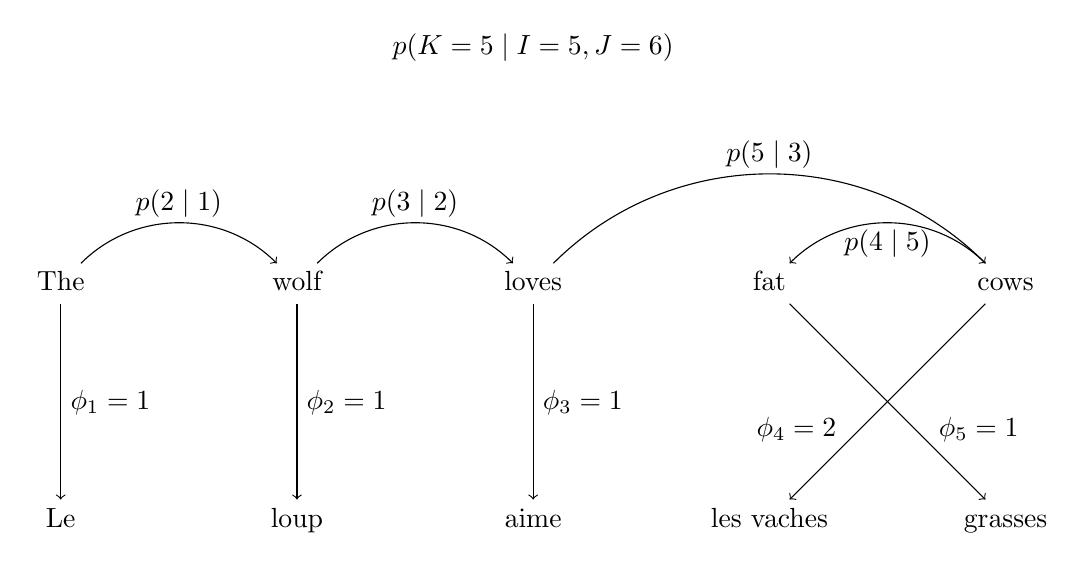
\begin{tikzpicture} [node distance = 3cm, text height=1.5ex, text depth = .25ex, auto]
    % place nodes
    \node (the) {The};
    \node [right of = the] (wolf) {wolf};
    \node [right of = wolf] (loves) {loves};
    \node [right of = loves] (fat) {fat};
    \node [right of = fat] (cows) {cows};
    \node [above of = loves] (chooseSeg) {$p(K = 5 \mid I = 5, J = 6)$};
    
    \node [below of = the] (le) {Le};
    \node [below of = wolf] (loup) {loup};
    \node [below of = loves] (aime) {aime};
    \node [below of = fat] (lesVaches) {les vaches};
    \node [below of = cows] (grasses) {grasses};

    % draw edges
    \draw [->] (the) to node {$\phi_1 = 1$} (le);
    \draw [->] (wolf) to node {$\phi_2 = 1$} (loup);
    \draw [->] (loves) to node {$\phi_3 = 1$} (aime);
    \draw [->] (fat) to node [right, xshift = 1.5em, yshift = -1em] {$\phi_5 = 1$} (grasses);
    \draw [->] (cows) to node [left, xshift = -1.5em, yshift = -1em] {$\phi_4 = 2$} (lesVaches);

    \draw [->] (the) to [bend left = 45] node {$p(2 \mid 1)$} (wolf);
    \draw [->] (wolf) to [bend left = 45] node {$p(3 \mid 2)$} (loves);
    \draw [->] (loves) to [bend left = 45] node {$p(5 \mid 3)$} (cows);
    \draw [->] (cows) to [bend right = 45] node {$p(4 \mid 5)$} (fat);
  \end{tikzpicture}
  \end{center}
  \caption{Simplified generative story for an HMM word-to-phrase alignment model.
    Adapted from~\citep{deng-and-byrne:2008:ASLP}.
    The adjective noun sequence \emph{fat cows} is
    reordered into the noun adjective sequence \emph{vaches grasses}.
    The word \emph{cows} has fertility 2 as it is translated
    into the target phrase \emph{les vaches}.}
  \label{fig:wordtophrase}
\end{figure}

\subsection{Symmetrisation Heuristics}
\label{sec:symmetrisationHeuristics}

We have mentioned that the IBM and HMM alignment models
are not symmetric: they only allow a many-to-one mapping from
source words to target words.
In order to address this issue, one can train
alignment models in both source-to-target and target-to-source
directions, obtain Viterbi alignments from
both models and apply symmetrisation
strategies~\citep{och-tillmann-ney:1999:EMNLP,och-ney:2003:CL,koehn-och-marcu:2003:NAACL}.
\citet{och-tillmann-ney:1999:EMNLP} designed
a first symmetrisation heuristic that was later on dubbed
as the \emph{grow} heuristic. \citet{koehn-och-marcu:2003:NAACL}
later extended the \emph{grow} heuristic into
the \emph{grow-diag} and \emph{grow-diag-final} heuristics
and examined the impact on translation
performance for each heuristic.

Alignments from source to target (i.e. in which the alignment is
a function from source positions to target positions)
and target to source are denoted
$\bm{a}_{f2e}$ and $\bm{a}_{e2f}$ respectively.
Let us consider a sentence pair $(\bm{f}, \bm{e})$, and
source-to-target and target-to-source Viterbi alignments
$\bm{a}_{f2e}$ and $\bm{a}_{e2f}$.
The \emph{intersection} and \emph{union} heuristics
are defined as follows:
%
\begin{itemize}
  \item \emph{intersection}: $\bm{a} = \bm{a}_{e2f} \cap \bm{a}_{f2e}$
  \item \emph{union}: $\bm{a} = \bm{a}_{e2f} \cup \bm{a}_{f2e}$
\end{itemize}
%
The \emph{intersection} heuristics typically produces high precision alignments
while the \emph{union} heuristics typically produces high recall
alignments~\citep{och-ney:2003:CL}.
We now present the \emph{grow} heuristic and its variants, which are based
on the initial \emph{intersection} and \emph{union} heuristics.
The \emph{grow} heuristic algorithm is presented in
\autoref{alg:growHeuristic}. The input is a sentence
pair $(f_1^J, e_1^I)$, a source-to-target
alignment $\bm{a}_{f2e}$ and a target-to-source alignment
$\bm{a}_{e2f}$. The resulting alignment $\bm{a}$ is initialized
with the
intersection (\hyperlink{alg:line:initGrow}{line \ref{alg:line:initGrow}}).
Then alignment links that are in the union and that are neighbours of already existing
alignment links (\hyperlink{alg:line:neighbours}{line \ref{alg:line:neighbours}})
are considered. If the source or the target word is not already
aligned (\hyperlink{alg:line:notAlreadyAligned}{line \ref{alg:line:notAlreadyAligned}}),
then the link is added to the resulting
alignment (\hyperlink{alg:line:addLink}{line \ref{alg:line:addLink}}).
This is repeated until no more links are added.
%
\begin{figure}
  %\begin{footnotesize}
  \begin{algorithmic}[1]
    \Function{Grow}{$f_1^J, e_1^J, \bm{a}_{f2e}, \bm{a}_{e2f}$}
      \State{$\bm{a} \gets \bm{a}_{f2e} \cap \bm{a}_{e2f}$} \hypertarget{alg:line:initGrow}{} \label{alg:line:initGrow}
      \While{\textbf{true}}
        \State{added $\gets$ \textbf{false}}
        \For{$i \in [1, I]$}
          \For{$j \in [1, J]$}
            \If{$(j, i) \in \bm{a}$}
            \For{$(k, l) \in $ \Call{Neighbours}{$(j,i)$} $\cap (\bm{a}_{f2e} \cup \bm{a}_{e2f})$} \hypertarget{alg:line:neighbours}{} \label{alg:line:neighbours}
              \If{$k$ not aligned in $\bm{a}$ \textbf{or} $l$ not aligned in $\bm{a}$} \hypertarget{alg:line:notAlreadyAligned}{} \label{alg:line:notAlreadyAligned}
                \State{$\bm{a} \gets \bm{a} \cup (k, l)$} \hypertarget{alg:line:addLink}{} \label{alg:line:addLink}
                \State{added $\gets$ \textbf{true}}
              \EndIf
            \EndFor
            \EndIf
          \EndFor
        \EndFor
        \If{not added} 
          \State{\textbf{break}}
        \EndIf
      \EndWhile
      \State{\Return $\bm{a}$}
    \EndFunction
  \end{algorithmic}
  %\end{footnotesize}
  \caption{Algorithm for the \emph{grow} symmetrisation
    heuristic~\citep{koehn:2010:book}.
    The alignment is initialized from the intersection and alignment links
    that are neighbours to existing alignment links are iteratively added if the source
    or the target is not already aligned.}
  \label{alg:growHeuristic}
\end{figure}

In the \emph{grow} heuristic, neighbours are defined as horizontal or
vertical neighbours. If diagonal neighbours are also considered, then
the heuristic becomes \emph{grow-diag}. The \emph{grow} heuristic
also has an optional step called \emph{final}. Alignment
links in the union where the source or the target is not already
aligned can also be added to the resulting alignment. If only links
in the union where the source \emph{and} the target are not already
aligned are considered for the \emph{final} procedure, then
the optional step is called \emph{final-and}.

Symmetrisation heuristics have been shown to be beneficial for
alignments both in terms of alignment quality as measured
by comparing automatic alignments to human alignments and
in translation quality when alignments are used as an
intermediate step in the translation pipeline.

%
%Symmetrised alignments have be shown to produce better translation results than
%unidirectional alignments. However, we find in one of our experiments that this
%is not always the case (see \autoref{sec:extractionFromPosteriorsSymmetrising}).

% This should review phrase based SMT.
% Why: the gyro decoder is like a phrase based SMT decoder.

% phrase based extraction + stack base decoding

\section{Log-Linear Model of Machine Translation}
\label{sec:loglinearModel}

%notes on adam berger paper
%model conditional prob
%p(y | x): x is phrase containing word "in", y is translation of "in"
%collect stats ptilda(x, y)
%binary feature: f(x, y) = 1 if y = en and April follows in
%expected value of f: ptilda(f) = sum_x,y ptilda(x,y) f(x,y)
%p(f) = sum_x,y ptilda(x) p(y | x) f(x,y)
%constraint: p(f) = ptilda(f)
%max entropy principle: choose p that satisfies the constraints
%and that maximizes entropy
%H(p) = -sum_x,y ptilda(x) p(y|x) log p(y|x)
%use Lagrange multiplier and Kuhn Tucker theorem to find that the solution
%is p(y|x) propto exp(\sum lambda_i f_i(x,y)). find lambda by max dual problem.
%also: p that satisfies constr and max entropy is also the
%p in the parametric family ... that maximizes likelihood of training sample.
%application to Candide.
%use max entropy modelling to predict translation of word in context.
%use max entropy modelling to predict word order.
%use max entropy modelling to segment.
%context dependent translation:
%first viterbi align training. then create events (x,y) (6 words
%surrounding in)
%incorporate this context dep translation into general translation model.

As we have seen in \autoref{sec:sourceChannelModel}, SMT was historically
framed as a source-channel model. As an alternative,
\citet{berger-dellapietra-dellapietra:1996:CL} introduce maximum entropy
models for natural language processing. In maximum entropy modelling, we
wish to estimate a conditional probability $p(\bm{y} \mid \bm{x})$.
Given a training sample, various feature functions deemed to be relevant
are picked. We then constrain $p$ such that the expected value of each
feature function $f$ with respect to the empirical distribution is equal
to the expected value of $f$ with respect to the model $p$. Finally, $p$
is chosen among all models that satisfy the constraints defined by the
features and such that its entropy is maximum.
\citet{berger-dellapietra-dellapietra:1996:CL} show how a maximum entropy
model can be parameterized as an exponential, or log-linear model. They
apply this model to three machine translation related tasks. First, they
use a maximum entropy model to predict the translation of a word using
the context for that word. Then, they use a maximum entropy model to
predict the target language word order. Finally, they apply maximum
entropy modelling in order to predict the source sentence segmentation.

%notes och and ney 2002
%search done by the maximum approximation
%first present log linear model
%log linear model generalization of source channel model
%log linear model presented with additional alignment variable
%p(e_1^I, a_1^J | f_1^J) propto exp(sum_1^M lambda_m h_m(e_1^I, f_1^J, a_1^J))
%alignment template model
%p(f_1^J | e_1^I) = sum_{z_1^K, a_1^K} p(a_1^K | e_1^I) . p(z_1^K | a_1^K, e_1^I) . p(f_1^J | z_1^K, a_1^K, e_1^I)
%each component modeled with max entropy model

\citet{och-tillmann-ney:1999:EMNLP} notice that using an erroneous
version of the source-channel model, that is using the following equation:
%
\begin{equation}
  \bm{\hat{e}} = \argmax_{\bm{e}} p(\bm{e} \mid \bm{f}) \, p(\bm{e})
\end{equation}
%
gives comparable performance with respect to using the correct
formulation of the source-channel model given in \autoref{eq:noisy}.
Then \citet{och-ney:2002:ACL} propose the following log-linear model extension:
%
\begin{align}
  \bm{\hat{e}} &= \argmax_{\bm{e}} p(\bm{e} \mid \bm{f}) \nonumber \\
               &= \argmax_{\bm{e}} \frac{\exp(\sum_{m=1}^M \lambda_m h_m(\bm{e}, \bm{f}))}{\sum_{\bm{e'}}\exp(\sum_{m=1}^M \lambda_m h_m(\bm{e'}, \bm{f}))} \nonumber \\
               &= \argmax_{\bm{e}} \exp(\sum_{m=1}^M \lambda_m h_m(\bm{e}, \bm{f})) \label{eq:loglinearModel}
\end{align}
%
where $h_m$ are called \emph{feature functions} and $\lambda_m$
are called \emph{feature weights}. The log-linear model is an extension
to the source-channel model because it can be reduced to the original
source-channel model with the following settings:
%
    \begin{itemize}
      \item $M = 2$
      \item $h_1(\bm{e}, \bm{f}) = \log (p(\bm{f}|\bm{e}))$
      \item $h_2(\bm{e}, \bm{f}) = \log (p(\bm{e}))$
      \item $\lambda_1 = \lambda_2 = 1$
    \end{itemize}
%
Log-linear models were originally trained with the maximum likelihood
criterion, which precisely makes them equivalent to maximum entropy
models~\citep{berger-dellapietra-dellapietra:1996:CL}. However,
more effective training techniques such as minimum error rate
training~\citep{och:2003:ACL} were introduced subsequently, that do
not require the computation of a normalization constant
(see \autoref{sec:mert}).
Thus, in practice, SMT models are effectively simply linear models, with the objective
function presented in \autoref{eq:linearModel}:
%
\begin{equation}
  \bm{\hat{e}} = \argmax_{\bm{e}} \sum_{m=1}^M \lambda_m h_m(\bm{e}, \bm{f})
  \label{eq:linearModel}
\end{equation}

%In practice, \citet{och-ney:2002:ACL} do not use \autoref{eq:loglinearModel}.
%They introduce several latent variables in a so called \emph{alignment template}
%approach. The translation model is defined in \autoref{eq:alignmentTemplate}:
%
%\begin{equation}
%  p(e_1^I \mid f_1^J) = \sum_{z_1^K, a_1^K} p(a_1^K \mid e_1^I) p(z_1^K \mid a_1^K, e_1^I) p(f_1^J \mid z_1^K, a_1^K, e_1^I)
%  \label{eq:alignmentTemplate}
%\end{equation}
%
% TODOFINAL check if it is "correct" to invert the notation in above equation wrt to original publication
%where the variables $z_1^K$ and $a_1^K$ are alignment templates and the alignment of alignment templates.
%Each term in \autoref{eq:alignmentTemplate} is modelled as a maximum entropy model and search
%is carried out using the maximum approximation defined in \autoref{eq:maxApproximation}:
%
% TODONEVER finish this
%\begin{align}
%  \hat{e_1^I} &= \argmax_{z_1}
%  \label{eq:maxApproximation}
%\end{align}

% TODONEVER talk about training methods: GIS vs MERT

\section{Phrase-Based Translation}
\label{sec:phraseBasedTranslation}

%notes on och et al 1999
%compare word based and phrase based
%e = argmax p(e) p(f|e)
%word based model: each source word (french) assigned exactly one target word (english)
%difficult to model context and also to translate compound words
%model two alignment levels: phrase level alignment between phrases and word level alignment between words within phrases
%word based approach: use an HMM
%p(f_1^J | e_1^I) = sum_{a_1^J} prod_j p(a_j | a_{j - 1}) p(f_j | e_{a_j})
%some restrictions are used (so called monotonicity): alignment jump between a_{j - 1} and a_j can only be 0, 1, 2.
%Q_{e'}(j, e): probability of best partial hypothesis (e_1^i, a_1^j) with e_i = e, e_{i - 1} = e' and a_j = i
%search: mapping j -> (a_j, e_{a_j})
%DP recursion:
%Q_e'(j, e) = p(f_j | e) . max {
%  p(0) . Q_e'(j - 1, e),
%  p(1) . max_e'' {p(e | e', e'') Q_e''(j - 1, e')},
%  p(2) . max_{e'', e'''} {p(e | e', e'') . p(e' | e'', e''') . Q_e'''(j - 1, e'')}
%  }
%optimal translation: max_e',e Q_e'(J, e) . p(\$ | e, e')
%extension to one-to-many alignment model.
%solution: reverse translation direction, then extend English vocab with multiple words, then redo standard training for original translation direction.
%alignment template approach
%problem with word based models: only allow one to many or many to one, or many to many but hacky solution
%model phrase to phrase is a way to model context.
%alignment template z: triple (Ftilda, Etilda, Atilda) alignment Atilda between source class sequence Ftilda and
%target class sequence Etilda.
%Atilda: matrix with binary values
%Atilda allows for many to many
%Ftilda and Etilda automatically trained bilingual classes
%use classes for better generalization
%alignment template applicable to sequence source words ftilda if
%alignment template classes and classes of source words are equal
%application of alignment template contraints the target words to have the right classes
%selection target words: p(etilda | z, ftilda)
%p(ftilda | (Ftilda, Etilda, Atilda), etilda) = delta(classes(etilda), Etilda) delta(classes(ftilda), Ftilda) prod_{j=1}^J (I???) p(f_j | Atilda, etilda)
%p(f_j | Atilda, etilda) = sum_{i = 0}^I p(i | j; Atilda) p(f_j | e_i)
%p(i | j, Atilda) = Atilda(i, j) / (sum_i Atilda(i, j))
%rien compris
%phrase level alignment
%decompose f_1^J and e_1^I into sequence of phrases
%f_1^J = ftilda_1^K
%assume that there is only one possible segmentation (possibly one of the differences between Och and Koehn)
%p(f_1^J | e_1^I) = p(ftilda_1^K | etilda_1^K)
%                 = sum_{atilda_1^K} p(atilda_1^K, ftilda_1^K | etilda_1^K)
%                 = sum_{atilda_1^K} p(atilda_1^K | etilda_1^K) p(ftilda_1^K | atilda_1^K, etilda_1^K)
%                 = sum_{atilda_1^K} prod_{k = 1}^K p(atilda_k | atilda_1^{k-1}, K) p(ftilda_k | etilda_{atilda_k})
%p(ftilda | etilda) = sum_z p(z| etilda) p(ftilda | z, etilda)
%training: s2t and t2s hmm without the max approximation
%get the viterbi alignments a_1^J and b_1^I
%use the grow diag symmetrisation heuristic.
%estimate bilingual word lexicon p(f|e): n_A(f, e) | n(e)
%train world classes
%extract consistent phrase pairs from alignment
%obtain n(z) of how often alignment template occurs in aligned corpus.
%relative freq estimate: p(z = (Ftilda, Etilda, Atilda) | etilda) = n(z) . delta(classes(etilda), Etilda) / n(classes(etilda))
%decoding search
%objective: argmax_{e_1^I} p(e_1^I p(e_1^I | f_1^J)) (wrong version of source channel model)
%use class-based 5g lm
%preprocessing before translation: filter alignment templates per source sentence, segment source sentence
%segmentation objective: argmax_{ftilda_1...ftilda_k = f_1^J} prod_{k=1}^K max_z p(z | ftilda_k)
%search: produce partial hypotheses with info: last target word, language model state,
%source coverage, last alignment template, position of last target word in alignment template
%instantiation (???), cost so far, backpointer
%integrate future cost because compare hypotheses that cover different parts of the input

%notes on och-ney 2004 (journal paper version of och et al. 1999)
%overview: align, extract, extracted phrases with alignment and word classes are
%called alignment templates
%log-linear model: hat{e_1^I} = argmax_{e_1^I} p(e_1^I | f_1^J)
%                             = argmax exp(sum_m=1^M lambda_m h_m(e_1^I, f_1^J))/Z
%parameters lambda trained with MLE (same as maximum entropy)
%or trained with MERT
%use latent variable
%p(e_1^I, a_1^J | f_1^J) = (1/Z) . exp(sum_1^M lambda_m h_m(e_1^I, f_1^J, a_1^J))
%description of word alignments etc.
%description of symmetrisation heuristics etc.
%symmetrized Viterbi alignments used to compute translation lexicon
%description of phrase-extract
%alignment templates: replace words with word classes and store
%alignment info for each phrase pair
%alignment template z = (F_1^J', E_1^I', Atilda)
%F_1^J' source class sequence
%E_1^I' target class sequence
%Atilda: alignment between source class seq and target class seq
%automatically train bilingual classes
%notation: etilda, ftilda target and source phrases
%p(z = (F_1^J', E_1^I', Atilda) | ftilda) = N(z) . delta(F_1^J', C(ftilda)) / N(C(ftilda%))
%remove alignment templates with prob less than 0.01
%limit on source phrase: between 4 and 7
%translation model
%f_1^J = ftilda_1^K
%e_1^I = etilda_1^K
%model described for a specific segmentation but in search
%optimal segmentation also searched for
%pi_1^K: permutation of the phrases, models phrase reordering
%etilda_k is translation of ftilda_{pi_k}
%alignment template between f_{pi_k} and e_k: z_k
%hidden variables in the model: pi_1^K, z_1^K
%use log-linear model, feature functions depend on source, target and hidden variables
%features
%alignment template selection
%h_AT(e_1^I, f_1^J, pi_1^K, z_1^K) = log prod_1^K p(z_k | f_{j_{pi_k - 1} + 1}^{j_{pi_k}%})
%h_WRD(e_1^I, f_1^J, pi_1^K, z_1^K) = log prod_1^I p(e_i | {f_j, (i,j) in A}, E_i)
%p(e_i | {f_j, (i,j) in A}, E_i)
%etc etc. hyper complique
%h_AL phrase alignment (reordering model)
%h_AL(e_1^I, f_1^J, pi_1^K, z_1^K) = sum_{k=1}^{K+1} |j_{pi_k - 1} - j_{pi_{k - 1}}
%3gram lm + 5g class based lm
%training: blabla
%search
%breadth-first search with pruning: beam search
%search objective:
%hat{e_1^I} = argmax_{e_1^I} sum_{pi_1^K, z_1^K} p(e_1^I, z_1^K, pi_1^K | f_1^J)
%           ~~ argmax_{e_1^I, pi_1^K, z_1^K} p(e_1^I, z_1^K, pi_1^K | f_1^J)
%           = argmax_{e_1^I, pi_1^K, z_1^K} sum_{m = 1}^M lambda_m h_m(e_1^I, f_1^J, pi_%1^K, z_1^K)
%use the max approximation
%structure of search space
%generate hypothesis left to right on the target
%preprocessing step: first determine all source phrases that match an alignment template
%unknown words carried over
%use 5-best target words for each target class according to some criterion
%use hypothesis recombination
%pruning done for hypotheses that cover the same number of source words
%future cost estimation
%rien compris
%exps etc. etc.

%notes on phrase-based mt by koehn's book
%EM training of phrase-based models: NO
%Extensions to the Reordering Model
%zh-en, ar-en, fr-en in contrast to de-en or jp-en
%lexicalized reordering
%reordering model p_o predicts orientation m,s,d given phrase pair f,e:
%p_o(orientation | f, e)
%extract each phrase pair with orientation type p_o(orientation | f, e) = count(orientation, e, f) / sum_o count(o, e, f)
%to be smoothed with prior p_o(orientation)
%phrase translation as classification: use max ent model to model context
%use phrase penalty to model source segmentation
%use word penalty to model length
%lexical weighting a la koehn
%used as smoothing for translation model
%lex(e|f, a) = prod_{i = 1}^length(e) (1/|{j | (i,j) in a}|) sum_{j | (i,j) in a} w(e_i | f_j)
%if english word unaligned, use the NULL word on the f side
%w estimated with rel freq from aligned corpus.
%use both lex(e|f,a) and lex(f|e,a)
%log linear model: TODONEVER find out what's the objective in moses/koehn2003
%phrase-extract etc. etc.
%source channel phrase-based model:
%e = argmax p(f|e) p(e)
%  = argmax prod_i p(f_i | e_i) d(start_i - end_{i - 1} -1)
%justification: segmentations are equally likely, max approximation ??
%d(x) propto alpha^|x|

%notes on phrase-based mt decoding by koehn's book
%description of hypothesis expansion
%computational complexity: NP complete/hard
%hypothesis recombination
%simple example: [it] [is] vs. [it is]
%more complicated example: [he] [does not] vs. [it] [does not]
%note: instead of deleting the hyp, we still keep pointer
%so that we can output n-best
%stack decoding
%stack <-> number of foreign words translated
%problem: some hyps in a stack cover different regions of the input
%histogram pruning and threshold pruning
%reordering limit in search
%future cost or outside cost or rest cost
%cost of translation option: translation cost easy,
%language model cost approximated by lm without context,
%reordering model ignored
%for each translation option, compute the ``cost without context''
%then estimate the cheapest cost for translating any span in the
%input using DP
%use future cost in search: add the cost of the remaining (gappy) span
%to the partial cost

%notes on koehn et al 2003
%"Note that phrase translation with a lexical weight is a
%special case of the alignment template model [Och et al.,
%1999] with one word class for each word."

So far, we have presented two modelling approaches to machine translation:
the original source-channel model and the current log-linear model. We also
have presented word alignment models, which were introduced within the source-channel
model framework and which are instances of word-based models.

% TODOFINAL motivation for phrase based: word based a:[1,J]->[1,I] so many to one mapping only
In the phrase-based translation paradigm, the minimal unit of translation consists
of phrases. Phrases are sequences of consecutive words, that need not be syntactically
or semantically motivated, but nevertheless are used as translation unit.
Benefits of phrase-based models include:
%
\begin{itemize}
  \item effectively disambiguating the translation of a word in a certain local context;
  \item effective local reordering within a phrase such as the adjective-noun inversion from French to English;
  \item effective translation of multi-word expressions, such as idioms.
\end{itemize}
%
Phrase-based models
currently achieve state-of-the-art performance for
certain language pairs that do not involve much reordering
such as French-English. They can be defined
in the source-channel model framework (see \autoref{sec:sourceChannelModel}) or
the log-linear model framework (see \autoref{sec:loglinearModel}).
Because the source-channel model is no longer widely used anymore and because it is
a special case of a log-linear model, we will focus our presentation
on the log-linear model.

There are different variations on the phrase-based translation paradigm.
We will focus on two popular approaches, namely the alignment template
model~\citep{och-tillmann-ney:1999:EMNLP,och-ney:2004:CL} and the phrase-based
model~\citep{koehn-och-marcu:2003:NAACL,koehn:2010:book}.

\subsection{Alignment Template Model}

The alignment template model uses the log-linear model presented
in \autoref{eq:loglinearModel} as a starting point and repeated in
\autoref{eq:loglinearModelRepeated}:
%
\begin{equation}
  \bm{\hat{e}} = \argmax_{e_1^J} \exp(\sum_{m = 1}^M \lambda_m h_m(f_1^J, e_1^I))
  \label{eq:loglinearModelRepeated}
\end{equation}
%
In order to reduce the number of parameters, two latent variables $\pi_1^K$
and $z_1^K$ are introduced. $z_1^K$ is a sequence of \emph{alignment templates}
while $\pi_1^K$ is a permutation of size $K$. An alignment template
is a triple $(\tilde{F}, \tilde{E}, \tilde{A})$ where $\tilde{F}$ is a
sequence of source word classes, $\tilde{E}$ is a sequence of target
word classes and $\tilde{A}$ is an alignment between $\tilde{F}$
and $\tilde{E}$. $\pi_1^K$ together with $z_1^K$ define
a source segmentation of $f_1^J$ into source phrases $\tilde{f}_1^K$,
a target segmentation of $e_1^I$ into target phrases $\tilde{e}_1^K$ and
a bijective mapping between source phrases and target phrases where
$\tilde{f}_{\pi_k}$ is mapped to $\tilde{e}_{k}$ for $k \in [1,K]$.
The alignment templates $z_1^K$ are constrained in such a way that
the alignment template classes match the word classes.
The alignment template translation model is summarized
in \autoref{fig:alignmentTemplateTranslationModel}.
%
\begin{figure}
  \begin{center}
    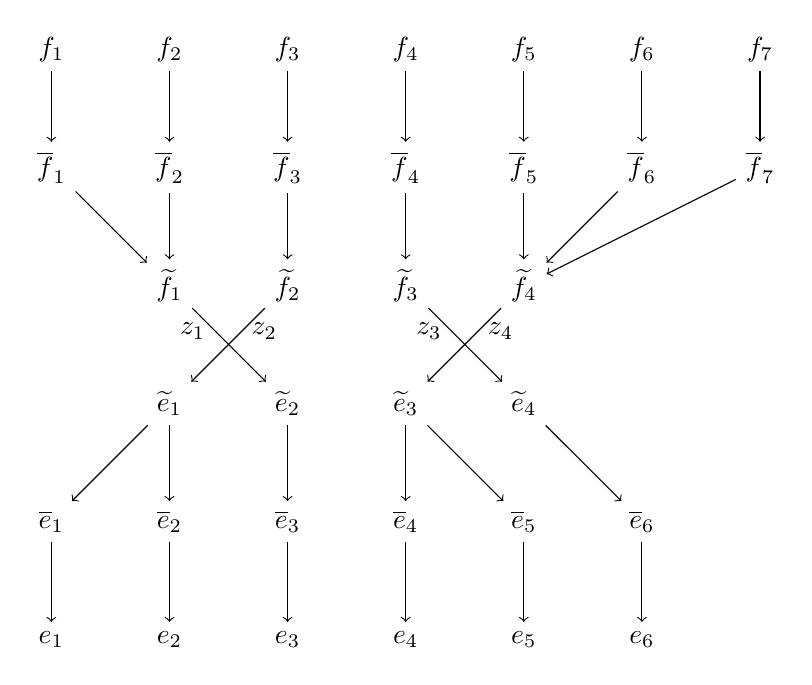
\begin{tikzpicture}[node distance = 1.5cm]
      % place nodes
      \node (f1) {$f_1$};
      \node (f2) [right of = f1] {$f_2$};
      \node (f3) [right of = f2] {$f_3$};
      \node (f4) [right of = f3] {$f_4$};
      \node (f5) [right of = f4] {$f_5$};
      \node (f6) [right of = f5] {$f_6$};
      \node (f7) [right of = f6] {$f_7$};

      \node (cf1) [below of = f1] {$\overline{f}_1$};
      \node (cf2) [below of = f2] {$\overline{f}_2$};
      \node (cf3) [below of = f3] {$\overline{f}_3$};
      \node (cf4) [below of = f4] {$\overline{f}_4$};
      \node (cf5) [below of = f5] {$\overline{f}_5$};
      \node (cf6) [below of = f6] {$\overline{f}_6$};
      \node (cf7) [below of = f7] {$\overline{f}_7$};

      \node (pf1) [below of = cf2] {$\widetilde{f}_1$};
      \node (pf2) [below of = cf3] {$\widetilde{f}_2$};
      \node (pf3) [below of = cf4] {$\widetilde{f}_3$};
      \node (pf4) [below of = cf5] {$\widetilde{f}_4$};

      \node (pe1) [below of = pf1] {$\widetilde{e}_1$};
      \node (pe2) [below of = pf2] {$\widetilde{e}_2$};
      \node (pe3) [below of = pf3] {$\widetilde{e}_3$};
      \node (pe4) [below of = pf4] {$\widetilde{e}_4$};

      \node (ce2) [below of = pe1] {$\overline{e}_2$};
      \node (ce1) [left of = ce2] {$\overline{e}_1$};
      \node (ce3) [below of = pe2] {$\overline{e}_3$};
      \node (ce4) [below of = pe3] {$\overline{e}_4$};
      \node (ce5) [below of = pe4] {$\overline{e}_5$};
      \node (ce6) [right of = ce5] {$\overline{e}_6$};

      \node (e1) [below of = ce1] {$e_1$};
      \node (e2) [below of = ce2] {$e_2$};
      \node (e3) [below of = ce3] {$e_3$};
      \node (e4) [below of = ce4] {$e_4$};
      \node (e5) [below of = ce5] {$e_5$};
      \node (e6) [below of = ce6] {$e_6$};
      % draw edges
      \draw [->] (f1) -- (cf1);
      \draw [->] (f2) -- (cf2);
      \draw [->] (f3) -- (cf3);
      \draw [->] (f4) -- (cf4);
      \draw [->] (f5) -- (cf5);
      \draw [->] (f6) -- (cf6);
      \draw [->] (f7) -- (cf7);

      \draw [->] (cf1) -- (pf1);
      \draw [->] (cf2) -- (pf1);
      \draw [->] (cf3) -- (pf2);
      \draw [->] (cf4) -- (pf3);
      \draw [->] (cf5) -- (pf4);
      \draw [->] (cf6) -- (pf4);
      \draw [->] (cf7) -- (pf4);

%      \draw[->] (P) to node {$\pi_{j}$} (B);

      \draw [->] (pf1) to node[left, xshift = -0.5em, yshift = 0.5em]{$z_1$} (pe2);
      \draw [->] (pf2) to node[right, xshift = 0.5em, yshift = 0.5em]{$z_2$} (pe1);
      \draw [->] (pf3) to node[left, xshift = -0.5em, yshift = 0.5em]{$z_3$} (pe4);
      \draw [->] (pf4) to node[right, xshift = 0.5em, yshift = 0.5em]{$z_4$} (pe3);

      \draw [->] (pe1) -- (ce1);
      \draw [->] (pe1) -- (ce2);
      \draw [->] (pe2) -- (ce3);
      \draw [->] (pe3) -- (ce4);
      \draw [->] (pe3) -- (ce5);
      \draw [->] (pe4) -- (ce6);

      \draw [->] (ce1) -- (e1);
      \draw [->] (ce2) -- (e2);
      \draw [->] (ce3) -- (e3);
      \draw [->] (ce4) -- (e4);
      \draw [->] (ce5) -- (e5);
      \draw [->] (ce6) -- (e6);
    \end{tikzpicture}
  \end{center}
  \caption{Alignment template translation process.
    Adapted from~\citep{och-ney:2004:CL}. The source word
  sequence $f_1^7$ is first transformed into a source class
  sequence $\overline{f}_1^7$. The source classes are then segmented
  into source phrases $\widetilde{f}_1^4$. The source phrases are then
  reordered and aligned to target phrases $\widetilde{e}_1^4$.
  For example, the source phrase $\widetilde{f}_1$ is aligned to
  the target phrase $\widetilde{e}_2$ through $z_1$.
  This means that the permutation $\pi_1^4$
  has value $\pi_2 = 1$. This also means that $z_1$
  define a word alignment between the source words $f_1$ and $f_2$
  and the target word $e_3$. Finally, the target
  phrases $\widetilde{e}_1^4$, which encode the target class sequence
  $\overline{e}_1^6$ generate the target word sequence $e_1^6$.}
  \label{fig:alignmentTemplateTranslationModel}
\end{figure}

Using the max approximation and making the feature
functions depend on the hidden variables, the translation model
can be rewritten in \autoref{eq:alignmentTemplateModel}:
%
\begin{equation}
  \bm{\hat{e}} = \argmax_{e_1^J, z_1^K, \pi_1^K} \exp(\sum_{m = 1}^M \lambda_m h_m(f_1^J, e_1^I, \pi_1^K, z_1^K))
  \label{eq:alignmentTemplateModel}
\end{equation}
%

% lexical feature in alignment template model
% symmetrized Viterbi alignments are used to compute a translation lexicon with relative frequency
% pi_1^K, z_1^K define an alignment between source and target: alignment A
% e_i has class E_i
% h_wrd(e_1^I, f_1^J, pi_1^K, z_1^K) = log prod_i=1^I p(e_i | {f_j | (i,j) in A}, E_i)
% p(e_i | {f_j | (i,j) in A}, E_i) = sum_{j | (i,j) in A} p(e_i | f_j) / |{j, (i,j) in A}| . delta(C(e_i), E_i)

\subsection{Phrase-Based Model}

The phrase-based model is similar to the alignment template
model but does not make use of source and target word classes.
Again, we use the latent variables $\pi_1^K$ and $z_1^K$.
This time, $z_k$ is defined as a triple $(\tilde{f}, \tilde{e}, \tilde{A})$
where $\tilde{f}$ is a sequence of source words, $\tilde{e}$ is a sequence
of target words and $\tilde{A}$ is an alignment between the words in $\tilde{f}$ and $\tilde{e}$.
The reason for using the alignment information between phrase pairs is to be able
to compute the lexical feature (see \autoref{sec:features}).
Because the lexical feature can be computed
by other means than this alignment
information (see again \autoref{sec:features}), it is also possible to simply
define $z_k$ as a phrase pair.

We have presented two variants of the phrase-based model. We will now
describe how to obtain the phrase pairs used for the latent variable $z$.

\subsection{Phrase Pair Extraction}
\label{sec:phrasextract}

A preliminary step to phrase pair extraction
is to obtain word aligned parallel text.
One possibility is to train source-to-target and
target-to-source word alignment models, obtain
Viterbi alignments in both directions, and
apply symmetrisation heuristics, as described
in \autoref{sec:symmetrisationHeuristics}.
Then phrase pairs are extracted from each
word aligned sentence pair.

Let us consider a sentence pair $(\bm{f},\bm{e})$ and an alignment $\bm{a}$.
We extract all phrase pairs that are {\em consistent} with the alignment.
This means that we extract all phrase pairs $(f_{j_1}^{j_2},e_{i_1}^{i_2})$ that
satisfy \autoref{eq:consistent} and \autoref{eq:atLeastOneLink}:
%
\begin{align}
  & \forall (j, i) \in \bm{a}, (j \in [j_1, j_2] \Leftrightarrow i \in [i_1,i_2]) \label{eq:consistent} \\
  & [j_1, j_2] \times [i_1, i_2] \cap \bm{a} \neq \emptyset \label{eq:atLeastOneLink}
\end{align}
%
\autoref{eq:consistent} requires that no alignment link be between a word
inside the phrase pair and a word outside the phrase pair.
\autoref{eq:atLeastOneLink} requires that there be at least one alignment link
between a source word in the source phrase and a target word in the target phrase.
For example, in \autoref{fig:ruleextract}, the phrase pair
$\langle$\emph{El mundo}, \emph{The world}$\rangle$ is extracted while the
phrase pair $\langle$\emph{es grande}, \emph{big}$\rangle$ is not
because the word \emph{es} (\emph{is}) is aligned
outside the phrase pair. Note that the consistency constraint
sometimes refers to only \autoref{eq:consistent} rather
than both \autoref{eq:consistent} and \autoref{eq:atLeastOneLink}.
%
\begin{figure}
  \begin{center}
    \begin{tikzpicture} [node distance = 2cm, text height=1.5ex, text depth=.25ex]
      % place nodes
      \node (El) {El};
      \node [right of = El] (mundo) {mundo};
      \node [right of = mundo] (es) {es};
      \node [right of = es] (grande) {grande};
      \node [below of = El] (The) {The};
      \node [right of = The] (world) {world};
      \node [right of = world] (is) {is};
      \node [right of = is] (big) {big};
      % draw edges
      \draw (El) -- (The);
      \draw (mundo) -- (world);
      \draw (es) -- (is) coordinate[midway](middleEsIs);
      \draw (grande) -- (big);
      % draw blocks around nodes to indicate rules
      %\node [draw=green, fit= (mundo) (world), rounded corners=1mm] {};
      \node [draw=green, fit= (El) (mundo) (The) (world), inner sep=1em, rounded corners=1mm] {};
      \draw [red, rounded corners=1mm] ($(es) + (-0.7,0.3)$) -- ($(big) + (0.7,-1.1)$) -- ($(grande) + (0.7,0.3)$) -- cycle;
      \node [ellipse, draw=red, minimum height = 4em, fit= (middleEsIs)] {};
    \end{tikzpicture}
  \end{center}
  \caption{Rule extraction for a sentence pair.
    For example, the phrase (El mundo, The world) is extracted.
    The phrase pair (es grande, big) is not extracted because it is
    not consistent with the alignment.}
  \label{fig:ruleextract}
\end{figure}
    
\subsection{Phrase-Based Decoding}
\label{sec:phraseBasedDecoding}

%notes on knight 1999 NP complete
%blabla on cryptograph and pos tagging
%machine translation
%v total English words
%bigram source model with v^2 parameters
%substitution/permutation channel models
%parallel corpus (sentence length <= m)
%monolingual french (???) sentence (length <= m)
%e_i has fertility phi_i: parameter n(phi | e)
%french words produced according to s(f|e) and permuted according to d(j|i,m,l)
%model 1 EM training
%collect estimate epsilon(m | l) from data
%set s(f|e) uniform initially
%basically, decoding with M1 is NP-complete
%reduction from hamilton circuit

We have introduced two types of phrase-based
models and described a technique to extract
phrase-pairs, which are an essential component
of these models. We will now describe the decoding
process, which is an effective means to obtain
the optimal translation of a source sentence.

We first describe a naive strategy for decoding, in order
to motivate the need for a more efficient decoder.
A naive decoder may follow the following steps, given
a source sentence $\bm{f}$ of length $J$ to be translated:
%
\begin{itemize}
  \item Consider all possible segmentations of $\bm{f}$ into source phrases. There are $2^{J - 1}$ such segmentations.
  \item For each segmentation, consider all possible permutations of the source phrases. For a segmentation of size $K$, there are $K!$ such permutations.
  \item For each permutation of the source phrases, consider all translations of each source phrase, and concatenate the target
    phrases according to the permutation. The source phrases translations are given by the phrase pairs extracted from the training
    data (see \autoref{sec:phrasextract}). If there are 10 translations per source phrase, we obtain
    $10^K$ possible translation (for the segmentation and permutation considered).
  \item Rank the translations by their score and pick the highest scoring translation.
\end{itemize}
%
We can see that the search space is too large for this naive
approach to be feasible.
We now present a practical solution to the decoding process in phrase-based translation.
We will first introduce the translation process. Then, we will
describe how translation hypotheses are built incrementally.
We will then motivate the need for pruning and how pruning
is carried out. Finally, we will describe how future cost estimation
may reduce search errors.

\paragraph{Translation Process}

Given a source sentence, the translation process is to iteratively
pick a source phrase that has not been translated yet,
translate that source phrase into a target phrase
and append the target phrase to the translation, and repeat this
process until the source
sentence has been entirely covered by source phrases. While the process is not
complete, the concatenation of target phrases is called a
\emph{partial hypothesis}.

\paragraph{Hypothesis Expansion}

The decoding process starts from an initial empty partial hypothesis.
This empty partial hypothesis is extended by picking source phrases,
appending their translations to the empty hypothesis.
At this stage, we have obtained several partial hypotheses.
The partial hypotheses are repeatedly extended until
all source words have been covered.
Partial hypotheses are represented by states
that contain the information necessary to
compute the cost of an extension.
If we use an $n$-gram language model as a feature,
the state will encode the cost of the partial hypothesis
and the last $n - 1$ words of the partial hypothesis.

\paragraph{Hypothesis Recombination}
\label{sec:phraseBasedHypothesisRecombination}

When two partial hypotheses share the same $n - 1$
words, only the partial hypothesis with the lower
cost can lead to the best final hypothesis. Therefore,
the partial hypothesis with higher cost can be discarded, or
alternatively, it is possible to make these two partial
hypotheses share the same state for rescoring purposes.

\paragraph{Stack Based Decoding and Pruning}
\label{sec:phraseBasedPruning}

The decoding search space is very large
as seen above. Approximations
therefore need to be made for an effective search.
The partial hypotheses are grouped in \emph{stacks}
by the number of source words covered.
This allows pruning. Each time a hypothesis expansion produces a hypothesis that
belongs to a certain stack, that stack is pruned.
There are two commonly used types of pruning: histogram pruning and threshold
pruning. Histogram pruning enforces a maximum number
of partial hypotheses in each stack. Threshold pruning
examines the cost of the best partial hypothesis in a stack
and discards all partial hypotheses in that stack whose cost
is greater than the best cost plus a threshold.
Histogram pruning provides a simple guaranty in terms
of computational complexity. On the other hand, because it relies
on cost, threshold pruning ensures a consistent quality for partial
hypotheses that survive the pruning threshold.

\paragraph{Future Cost}
\label{sec:phraseBasedFutureCost}

Partial hypotheses that cover the same number of source
words are grouped together for pruning purposes. However,
their cost may not be directly comparable, for example
partial hypotheses that correspond to the translation of frequent
words in the source might have a smaller cost than partial hypotheses
that correspond to the translation of rare words in the source.
To address this issue, a future cost that represents how difficult it is
to translate the rest of the sentence is added to the model cost of each
partial hypothesis.

\section{Hierarchical Phrase-Based Translation}
\label{sec:hierarchicalPhraseBasedTranslation}

% TODOFINAL reread from here
% TODOSUBMIT or TODOFINAL rework outline:
% make a separate section on features after hiero section
% last subsection of hiero should be decoding with hifst

\begin{sloppy} % in this paragraph, word running into the right margin

In the previous section, we have described the
phrase-based translation paradigm.
In this section, we present the
hierarchical phrase-based translation
model. This model relies on the synchronous
context free grammar formalism. Reordering
between source and target languages is modelled
by the grammar rather than by an \emph{ad} \emph{hoc}
reordering model, although using both the grammar
and a reordering model may be
beneficial~\citep{huck-EtAl:2013:WMT}.
A closely related formalism, inversion
transduction grammars, was previously
introduced~\citep{wu:1995:IJCAI,wu:1997:CL}, however, because hierarchical
phrase-based grammar only contain lexicalized rules, translation decoding
is more practical.
An alternative to hierarchical phrase-based
translation that also models discontinuous
phrases but does not use the same grammar
formalism has also been introduced
recently~\citep{galley-manning:2010:NAACLHLT}.

\end{sloppy}

\subsection{Introduction and Motivation}
\label{sec:hierintro}

Phrase-based models generally impose a limit on the size
of the phrase pairs extracted while, in decoding, phrases
are typically reordered within a certain limit.
These restrictions may be problematic for language pairs
such as German-English or Chinese-English that allow
arbitrary reordering in some instances.
Hierarchical phrase-based translation was introduced
in order to overcome the reordering limitations from
phrase-based models~\citep{chiang:2005:ACL,chiang:2007:CL}.
For example, the Chinese sentence with English gloss
in \autoref{fig:exampleHiero} requires ``nested'' reordering~\citep{chiang:2007:CL}:
%
\begin{itemize}
  \item The phrase \emph{with North Korea have diplomatic relations} must be reordered into
    the phrase \emph{have diplomatic relations with North Korea}.
  \item The phrase \emph{few countries one of} must be reordered into the phrase \emph{one of (the) few countries}.
  \item After the two previous segments are reordered, \emph{have diplomatic relations with North Korea that one of the few countries} must be reordered into \emph{one of the few countries that have diplomatic relations with North Korea}.
\end{itemize}
%
\begin{CJK}{UTF8}{gbsn}
\begin{figure}
  \begin{center}
    \begin{footnotesize}
    \begin{tikzpicture} [node distance = 1.3cm]
      % place nodes
      \node (AustraliaZh) {澳洲};
      \node [right of = AustraliaZh](IsZh) {是};
      \node [right of = IsZh](WithZh) {与};
      \node [right of = WithZh](NorthKoreaZh) {北韩};
      \node [right of = NorthKoreaZh](HaveZh) {有};
      \node [right of = HaveZh](DiplomaticRelationsZh) {邦交};
      \node [right of = DiplomaticRelationsZh](ThatZh) {的};
      \node [right of = ThatZh](FewZh) {少数};
      \node [right of = FewZh](CountriesZh) {国家};
      \node [right of = CountriesZh](OneOfZh) {之一};

      \node [below of = AustraliaZh](AustraliaGloss) {Australia};
      \node [below of = IsZh](IsGloss) {is};
      \node [below of = WithZh](WithGloss) {with};
      \node [below of = NorthKoreaZh, align = left](NorthKoreaGloss) {North \\ Korea};
      \node [below of = HaveZh](HaveGloss) {have};
      \node [below of = DiplomaticRelationsZh, align = left](DiplomaticRelationsGloss) {diplomatic \\ relations};
      \node [below of = ThatZh](ThatGloss) {that};
      \node [below of = FewZh](FewGloss) {few};
      \node [below of = CountriesZh](CountriesGloss) {countries};
      \node [below of = OneOfZh, align = left](OneOfGloss) {one \\ of};

      \node [below = 4cm of AustraliaGloss](Australia) {Australia};
      \node [right of = Australia](Is) {is};
      \node [right of = Is, align = left](OneOf) {one \\ of};
      \node [right of = OneOf, align = left](Few) {the \\ few};
      \node [right of = Few](Countries) {countries};
      \node [right of = Countries](That) {that};
      \node [right of = That](Have) {have};
      \node [right of = Have, align = left](DiplomaticRelations) {diplomatic \\ relations};
      \node [right of = DiplomaticRelations](With) {with};
      \node [right of = With, align = left](NorthKorea) {North \\ Korea};

      % draw edges
      \draw (AustraliaGloss) -- (Australia);
      \draw (IsGloss) -- (Is);
      \draw (WithGloss) -- (With);
      \draw (NorthKoreaGloss) -- (NorthKorea);
      \draw (HaveGloss) -- (Have);
      \draw (DiplomaticRelationsGloss) -- (DiplomaticRelations);
      \draw (ThatGloss) -- (That);
      \draw (FewGloss) -- (Few);
      \draw (CountriesGloss) -- (Countries);
      \draw (OneOfGloss) -- (OneOf);
    \end{tikzpicture}
    \end{footnotesize}
  \end{center}
  \caption{Example of Chinese sentence that needs nested reordering in order to be translated into English.
  Adapted from \citep{chiang:2007:CL}.}
  \label{fig:exampleHiero}
\end{figure}
\end{CJK}  
%
Phrase-based systems can model this type of movement but
they require very long phrase pairs, which is
impractical to rely upon because of data sparsity. On the other
hand, hierarchical phrase-based grammars do model this type of movement using
shorter phrase pairs but with more complex rules.

\subsection{Hierarchical Grammar}
\label{sec:hiergrammar}

\subsubsection{Hierarchical Grammar Definition}

A hierarchical phrase-based grammar, or hierarchical grammar, or Hiero grammar,
which is a particular instance of a synchronous context free
grammar~\citep{lewis-stearns:1968:JACM,aho:1969:JCSS}, is
a set of rewrite rules of the following type:
%
\begin{equation}
  X \rightarrow \langle \gamma, \alpha, \sim \rangle \nonumber
\end{equation}
%
where $X$ is a nonterminal, $\gamma$ and $\alpha$ are sequences of terminals and nonterminals and $\sim$ is an alignment
between nonterminals. Terminals that appear in $\gamma$ are words in the source language while terminals that appear in $\alpha$ are
words in the target language. Nonterminals are chosen from a finite set disjoint from the set of terminals. The alignment between nonterminals
indicates which nonterminals in the source and target languages correspond to each other. The alignment $\sim$ can be written with 
a set of matching indices.

\subsubsection{Types of Rules}
\label{sec:hieroTypesOfRules}

A rule may or may not contain any nonterminals.
A rule without nonterminals (on the right hand side) is
called a \emph{phrase-based rule}. A rule with nonterminals
is called a \emph{hierarchical rule}.
A hierarchical grammar also usually contains the following rules
called \emph{glue} rules:
%
\begin{align}
  S \rightarrow& \langle X, X \rangle \nonumber \\
  S \rightarrow& \langle S X, S X \rangle \nonumber
\end{align}
%
with $S$ the start symbol. The first glue rule is necessary to
be able to start a derivation.
The second glue rule allows concatenation of phrase-based or
hierarchical rules.

% TODOFINAL mention reordering and monotone rules
%When introducing hierarchical phrase-based translation, we mentioned
%that reordering between source and target language is modeled
%by the hierarchical grammar.
%This is achieved by so-called \emph{monotone}
%and \emph{reordering} rules. By definition, phrase-based
%rules are monotone.
%A hierarchical rule with one nonterminal only is monotone
%
%A hierarchical rule is monotone if it has a monotone
%alignment between nonterminals. For example, the
%rule $X \rightarrow \langle \text{\emph{Buenas tardes }} X, \text{\emph{ Good afternoon }} X \rangle$

\subsubsection{Hierarchical Grammar Example}

Let us consider for example the grammar
in \autoref{fig:exampleHieroGrammar} where each rewrite rule is given a name $R_i$.
%
\begin{figure}
\begin{CJK}{UTF8}{gbsn}
  \begin{align}
    R_1:&\; S \rightarrow \langle X, X \rangle \nonumber \\
    R_2:&\; S \rightarrow \langle S X, S X \rangle \nonumber \\
    R_3:&\; X \rightarrow \langle X_1 \mbox{ 的 } X_2, \mbox{ the } X_2 \mbox{ that } X_1 \rangle \nonumber \\
    R_4:&\; X \rightarrow \langle X \mbox{ 之一}, \mbox{ one of } X \rangle \nonumber \\
    R_5:&\; X \rightarrow \langle \mbox{与 } X_1 \mbox{ 有 } X_2, \mbox{ have } X_2 \mbox{ with } X_1 \rangle \nonumber \\
    R_6:&\; X \rightarrow \langle \mbox{澳洲}, \mbox{ Australia} \rangle \nonumber \\
    R_7:&\; X \rightarrow \langle \mbox{是}, \mbox{ is} \rangle \nonumber \\
    R_8:&\; X \rightarrow \langle \mbox{北韩}, \mbox{ North Korea} \rangle \nonumber \\
    R_9:&\; X \rightarrow \langle \mbox{邦交}, \mbox{ diplomatic relations} \rangle \nonumber \\
    R_{10}:&\; X \rightarrow \langle \mbox{少数 国家}, \mbox{ few countries} \rangle \nonumber
  \end{align}
  \caption{Example of hierarchical grammar.
    Adapted from~\citep{chiang:2007:CL}. With this grammar, it
    is possible to obtain a derivation for the sentence pair
    from \autoref{fig:exampleHiero}.
    The derivation is shown in \autoref{fig:exampleHieroDerivation}.}
  \label{fig:exampleHieroGrammar}
\end{CJK}
\end{figure}
%
With this grammar, it is possible to write a derivation, i.e.\ a sequence of rules,
that rewrites the start symbol $S$ into the sentence pair presented in
\autoref{sec:hierintro}~\citep{chiang:2007:CL}.
For example we can apply the derivation $R_2,R_2,R_1,R_6,R_7,R_4,R_3,R_{10},R_5,R_9,R_8$ as
in \autoref{fig:exampleHieroDerivation}.
%
\begin{figure}
\begin{CJK}{UTF8}{gbsn}
  \begin{footnotesize}
    \begin{align}
      S \rightarrow&\; \langle S X, S X \rangle \nonumber \\
      \rightarrow&\; \langle S X_1 X_2, S X_1 X_2 \rangle \nonumber \\
      \rightarrow&\; \langle X_1 X_2 X_3, X_1 X_2 X_3 \rangle \nonumber \\
      \rightarrow&\; \langle \mbox{澳洲 } X_2 X_3, \mbox{Australia } X_2 X_3 \rangle \nonumber \\
      \rightarrow&\; \langle \mbox{澳洲 是 } X_3, \mbox{Australia is } X_3 \rangle \nonumber \\
      \rightarrow&\; \langle \mbox{澳洲 是 } X \mbox{ 之一}, \mbox{Australia is one of } X \rangle \nonumber \\
      \rightarrow&\; \langle \mbox{澳洲 是 } X_1 \mbox{ 的 } X_2 \mbox{ zhiyi}, \mbox{Australia is one of the } X_2 \mbox{ that } X_1 \rangle \nonumber \\
      \rightarrow&\; \langle \mbox{澳洲 是 } X_1 \mbox{ 的 少数 国家 之一}, \mbox{Australia is one of the few countries that } X_1 \rangle \nonumber \\
      \rightarrow&\; \langle \mbox{澳洲 是 与 } X_1 \mbox{ 有 } X_2 \mbox{ 的 少数 国家 之一}, \nonumber \\
      &\;                    \mbox{Australia is one of the few countries that have } X_2 \mbox{ with } X_1 \rangle \nonumber \\
      \rightarrow&\; \langle \mbox{澳洲 是 与 } X_1 \mbox{ 有 邦交 的 少数 国家 之一}, \nonumber \\
      &\;                    \mbox{Australia is one of the few countries that have diplomatic relations with } X_1 \rangle \nonumber \\
      \rightarrow&\; \langle \mbox{澳洲 是 与 北韩 有 邦交 的 少数 国家 之一}, \nonumber \\ 
      &\;                    \mbox{Australia is one of the few countries that have diplomatic relations with North Korea} \rangle \nonumber
    \end{align}
  \end{footnotesize}
  \caption{Example of hierarchical grammar derivation.
    Adapted from~\citep{chiang:2007:CL}.
    A derivation is simply a sequence of rules that
    rewrite the start symbol $S$ into a sentence pair.
    This particular derivation produces the sentence pair from \autoref{fig:exampleHiero}.} % TODOFINAL (done ?) better title, refer chiang and replace pinyin by chinese
  \label{fig:exampleHieroDerivation}
\end{CJK}
\end{figure}
%

\subsubsection{Constraints on Hierarchical Grammars}
\label{sec:constraintsOnHierarhicalGrammars}

The definition given for a hierarchical grammar is very general.
In practice, systems impose constraints on the types of rule the grammar contains
for efficiency reasons.
We first introduce the concept of rule
pattern~\citep{iglesias-degispert-banga-byrne:2009:EACL} in order
to describe these constraints in terms of patterns.
A rule pattern is simply a pair of regular expressions that match
the source and target sides of a hierarchical rule.
For example, the rule $X \rightarrow \langle \text{\emph{Buenas tardes }} X, \text{\emph{ Good afternoon }} X \rangle$
has a rule pattern $\langle \Sigma^+ X, \Psi^+ X \rangle$ where $\Sigma$ is the
source vocabulary and $\Psi$ is the target vocabulary.
For ease of notation, we use the notation $w$ for either $\Sigma^+$
or $\Psi^+$. Thus $w$ simply represents a sequence of terminals.
In our example, the pattern for the rule $ X \rightarrow \langle \text{\emph{Buenas tardes }} X, \text{\emph{ Good afternoon }} X \rangle$ is $\langle w X, w X \rangle$.
\citet{chiang:2007:CL} defines the following set of pattern-related constraints
that must be satisfied by the rules in a hierarchical grammar:
%
\begin{itemize}
  \item If a rule $X \rightarrow \langle \gamma, \alpha \rangle$ has a pattern $\langle w, w \rangle$, then $|\gamma| \leq 10$ and $|\alpha| \leq 10$.
  \item A rule $X \rightarrow \langle \gamma, \alpha \rangle$ must satisfy $|\gamma| \leq 5$.
  \item Rules have at most 2 nonterminals.
  \item The source side of a rule cannot have adjacent nonterminals.    
    \citet{setiawan-resnik:2010:NAACL} relax this constraint in order to model
    Chinese-English reordering phenomena that may be not always captured in
    training because of data sparsity.
    Note that the target side can still
    have adjacent nonterminals. % TODO ? for example see Section \ref{sec:emnlp10gramdef}.
  \end{itemize}
%
% TODOFINAL: missing constraints: boundary words, at least one alignment link
More fine-grained constraints can be defined on patterns.
For example, we use the configuration described
in \autoref{tab:patternconfig} for some of the translation experiments in this
thesis. This grammar was obtained following a greedy strategy of adding
in turn the most beneficial patterns for Arabic-English translation.

  \begin{table}[htbp]
    \begin{center}
      \footnotesize
      \begin{tabular}{|r@{ , }l|c||r@{ , }l|c|} \hline 
        {\bf \SR[source]} & {\bf\TR[target]} & {\bf include} & {\bf \SR[source]} & {\bf\TR[target]} & {\bf include} \\ \hline
        \SR[$w~X$] & \TR[$w~X$] & \textbf{no}  & \SR[$X~w$] & \TR[$w~X$] & yes \\
        \SR[$w~X$] & \TR[$X~w$] & yes &  \SR[$X~w$] & \TR[$w~X~w$] & yes \\
        \SR[$w~X$] & \TR[$w~X~w$] & yes  & \SR[$X~w$] & \TR[$X~w$] & \textbf{no} \\
        \hline
        \SR[$w~X~w$] & \TR[$w~X$] & yes &  \SR[$w~X~w$] & \TR[$X~w$] & yes \\
        \SR[$w~X~w$] & \TR[$w~X~w$] & yes &  \multicolumn{2}{|c|}{} & \\
        \hline
        \SR[$X1~w~X2$] & \TR[$w~X1~w~X2$] & \textbf{no} &  \SR[$X2~w~X1$] & \TR[$w~X1~w~X2$] & yes \\
        \SR[$X1~w~X2$] & \TR[$w~X1~w~X2~w$] & \textbf{no} &  \SR[$X2~w~X1$] & \TR[$w~X1~w~X2~w$] & yes \\
        \SR[$X1~w~X2$] & \TR[$w~X1~X2$] & \textbf{no} & \SR[$X2~w~X1$] & \TR[$w~X1~X2$] & yes \\
        \SR[$X1~w~X2$] & \TR[$w~X1~X2~w$] & \textbf{no} & \SR[$X2~w~X1$] & \TR[$w~X1~X2~w$] & yes \\
        \SR[$X1~w~X2$] & \TR[$X1~w~X2$] & \textbf{no} & \SR[$X2~w~X1$] & \TR[$X1~w~X2$] & yes \\
        \SR[$X1~w~X2$] & \TR[$X1~w~X2~w$] & \textbf{no} & \SR[$X2~w~X1$] & \TR[$X1~w~X2~w$] & yes \\
        \SR[$X1~w~X2$] & \TR[$X1~X2~w$] & \textbf{no} & \SR[$X2~w~X1$] & \TR[$X1~X2~w$] & yes \\
        \hline
        \SR[$w~X1~w~X2$] & \TR[$w~X1~w~X2$] & \textbf{no} & \SR[$w~X2~w~X1$] & \TR[$w~X1~w~X2$] & yes \\
        \SR[$w~X1~w~X2$] & \TR[$w~X1~w~X2~w$] & yes & \SR[$w~X2~w~X1$] & \TR[$w~X1~w~X2~w$] & yes \\
        \SR[$w~X1~w~X2$] & \TR[$w~X1~X2$] & yes & \SR[$w~X2~w~X1$] & \TR[$w~X1~X2$] & yes \\
        \SR[$w~X1~w~X2$] & \TR[$w~X1~X2~w$] & yes & \SR[$w~X2~w~X1$] & \TR[$w~X1~X2~w$] & yes \\
        \SR[$w~X1~w~X2$] & \TR[$X1~w~X2$] & yes & \SR[$w~X2~w~X1$] & \TR[$X1~w~X2$] & yes \\
        \SR[$w~X1~w~X2$] & \TR[$X1~w~X2~w$] & yes & \SR[$w~X2~w~X1$] & \TR[$X1~w~X2~w$] & yes \\
        \SR[$w~X1~w~X2$] & \TR[$X1~X2~w$] & yes & \SR[$w~X2~w~X1$] & \TR[$X1~X2~w$] & yes \\
        \hline
        \SR[$X1~w~X2~w$] & \TR[$w~X1~w~X2$] & yes & \SR[$X2~w~X1~w$] & \TR[$w~X1~w~X2$] & yes \\
        \SR[$X1~w~X2~w$] & \TR[$w~X1~w~X2~w$] & yes & \SR[$X2~w~X1~w$] & \TR[$w~X1~w~X2~w$] & yes \\
        \SR[$X1~w~X2~w$] & \TR[$w~X1~X2$] & yes & \SR[$X2~w~X1~w$] & \TR[$w~X1~X2$] & yes \\
        \SR[$X1~w~X2~w$] & \TR[$w~X1~X2~w$] & yes & \SR[$X2~w~X1~w$] & \TR[$w~X1~X2~w$] & yes \\
        \SR[$X1~w~X2~w$] & \TR[$X1~w~X2$] & yes & \SR[$X2~w~X1~w$] & \TR[$X1~w~X2$] & yes \\
        \SR[$X1~w~X2~w$] & \TR[$X1~w~X2~w$] & \textbf{no} & \SR[$X2~w~X1~w$] & \TR[$X1~w~X2~w$] & yes \\
        \SR[$X1~w~X2~w$] & \TR[$X1~X2~w$] & yes & \SR[$X2~w~X1~w$] & \TR[$X1~X2~w$] & yes \\
        \hline
        \SR[$w~X1~w~X2~w$] & \TR[$w~X1~w~X2$] & \textbf{no} & \SR[$w~X2~w~X1~w$] & \TR[$w~X1~w~X2$] & yes \\
        \SR[$w~X1~w~X2~w$] & \TR[$w~X1~w~X2~w$] & \textbf{no} & \SR[$w~X2~w~X1~w$] & \TR[$w~X1~w~X2~w$] & yes \\
        \SR[$w~X1~w~X2~w$] & \TR[$w~X1~X2$] & \textbf{no} & \SR[$w~X2~w~X1~w$] & \TR[$w~X1~X2$] & yes \\
        \SR[$w~X1~w~X2~w$] & \TR[$w~X1~X2~w$] & \textbf{no} & \SR[$w~X2~w~X1~w$] & \TR[$w~X1~X2~w$] & yes \\
        \SR[$w~X1~w~X2~w$] & \TR[$X1~w~X2$] & \textbf{no} & \SR[$w~X2~w~X1~w$] & \TR[$X1~w~X2$] & yes \\
        \SR[$w~X1~w~X2~w$] & \TR[$X1~w~X2~w$] & \textbf{no} & \SR[$w~X2~w~X1~w$] & \TR[$X1~w~X2~w$] & yes \\
        \SR[$w~X1~w~X2~w$] & \TR[$X1~X2~w$] & \textbf{no} & \SR[$w~X2~w~X1~w$] & \TR[$X1~X2~w$] & yes \\
        \hline
      \end{tabular}
    \end{center}
    \caption{Rule patterns included in a baseline hierarchical grammar.
      The decision whether to include each pattern was based on preliminary experiments
      in Arabic-English. Most beneficial patterns were added incrementally.}
    \label{tab:patternconfig}
  \end{table}
  
  Another restriction on hierarchical grammars is the extent of reordering allowed. \citet{degispert-iglesias-blackwood-banga-byrne:2010:CL} investigate the use
  of shallow-$N$ grammars that precisely control the depth of reordering in translation. We describe here 
  shallow-1 grammars~\citep{iglesias-degispert-banga-byrne:2009:EACL,degispert-iglesias-blackwood-banga-byrne:2010:CL} as
  they will be used for translation experiments in this thesis. Shallow-1 grammars
  allow only one level of reordering, they do not allow nested reordering as in the example presented in \autoref{sec:hierintro}.
  A shallow-1
  grammar is defined as follows:
%  
  \begin{align*}
    S &\rightarrow \langle X , X \rangle \\
    S &\rightarrow \langle S X , S X \rangle \\
    X &\rightarrow \langle \gamma_s , \alpha_s \rangle (\gamma_s, \alpha_s \in (T \cup \{V\})^{+}) \\
    X &\rightarrow \langle V , V \rangle \\
    V &\rightarrow \langle s , t \rangle (s \in T^{+}, t \in  T^{*})
  \end{align*}
%  
  where $S$ is the start symbol, $T$ is the set of terminals and $V$ is the set of nonterminals. There are two nonterminals
  apart from the start symbol: $X$ and $V$. The rule type $X \rightarrow \langle \gamma_s , \alpha_s \rangle$ corresponds
  to all hierarchical rules. It is possible to apply this type of rule only once in any derivation. Indeed, the
  right hand side contains only one type of nonterminal, $V$, which can be rewritten only with a phrasal rule corresponding
  to the line $V \rightarrow \langle s , t \rangle$. Note that for rules of the type $V \rightarrow \langle s , t \rangle$, $t$ can be
  the empty word, thus these rules, called {\em deletion rules}, allow deletion on the target side. Shallow-1 grammar are used for language pairs that do not present
  much reordering. Shallow-1 grammars were previously shown to work as well as full hierarchical grammars
  for the Arabic-English language pair~\citep{iglesias-degispert-banga-byrne:2009:EACL} and for
  the Spanish-English language pair~\citep{iglesias-degispert-banga-byrne:2009:SEPLN}.
  In addition, shallow-1 grammars reduce the search space of the decoder greatly, resulting in a much faster decoding
  time, a reduced memory use and potentially fewer search errors under the translation grammar.

  % TODOFINAL (?) log linear model for hpbt

    \subsection{Log-linear Model for Hierarchical Phrase-Based Translation} \label{sec:loglinear}

    We now define in more detail the log-linear model for hierarchical translation, which usually makes a maximum (max) approximation.
    We follow the original description~\citep{chiang:2007:CL}.
    For a sentence pair $(\bm{f}, \bm{e})$, let us define $\mathcal{D}$ the set of possible derivations $D$ of this sentence pair under 
    a hierarchical grammar. We will use the following notation for a derivation $D$:
    
    \begin{itemize}
%      \item $T$, the structure of the tree (that is the tree $D$ without leaves)
      \item the foreign yield $\bm{f}$. We define $f(D) = \bm{f}$
      \item the English yield $\bm{e}$. We define $e(D) = \bm{e}$
    \end{itemize}

    %Let us define $d = (T,{\bf f})$, so that we have $D = (d,{\bf e})$. 
    We can now derive the log-linear model for hierarchical translation:

    \begin{eqnarray}
      \bm{\hat{e}} &=& \argmax_{\bm{e}} p(\bm{e} \mid \bm{f}) \nonumber \\
                    &=& \argmax_{\bm{e}} \sum_{D \in \mathcal{D}} p(D,\bm{e} \mid \bm{f}) \mbox{ (marginalisation)} \nonumber \\
                    %&=& \argmax_{e} \sum_{d} p(d,{\bf e}|{\bf f}) \mbox{ (simply because the event D,{\bf e} is the same as the event d,{\bf e}} \\
                    &=& \argmax_{\bm{e}} \argmax_{D \in \mathcal{D}} p(D,\bm{e} \mid \bm{f}) \mbox{ (max approximation)} \nonumber \\
                    &=& e(\argmax_{{\bf e},D \in \mathcal{D}} p(D,{\bf e}|{\bf f})) \nonumber \\
                    &=& e(\argmax_{D | f(D) = {\bf f}} p(D))
    \end{eqnarray}

    Thanks to the max approximation, the distribution over derivations instead of the distribution over English
    sentences is modelled log-linearly and we obtain finally the following decoding equation:
%
    \begin{equation} \label{eq:decoding}
      \hat{{\bf e}} = e(\argmax_{D | f(D) = {\bf f}} \exp(\sum_{m=1}^M \lambda_m h_m(D)))
    \end{equation}
%
    One of the features, the language model, plays a particular role. The language model feature can be written as:
%    
    \begin{equation}
      h_M(D) = p_{LM}(e(D))
    \end{equation}
%
    where $M$ is the index of the language model feature, $p_{LM}$ is the language model and $e(D)$ is the English
    yield of the derivation $D$. It is not possible to compute the language model using dynamic programming since
    the language model needs context in order to be computed, therefore the language model feature is typically
    computed after a parsing step. % TODOFINAL explain better. for this, reread chiang's paper and/or hifst paper(s)
    
    Note that \autoref{eq:decoding} is an approximation and that there have been attempts to perform marginalisation over the latent variable 
    $D$ while keeping the translation process tractable~\citep{blunsom-cohn-osborne:2008:ACL,degispert-iglesias-blackwood-banga-byrne:2010:CL}.
    This can give gains over the max approximation, although subsequent rescoring
    steps (see \autoref{sec:rescoring}) can produce similar performance~\citep{degispert-iglesias-blackwood-banga-byrne:2010:CL}.

    %We now describe which features are used in our system, except for the language model which will be presented in Section \ref{lm}.

  \subsection{Rule Extraction} \label{sec:hierruleextract}

  We have so far given the definition of a hierarchical grammar and explained how it is used with statistical models.
  It is also necessary to extract an appropriate grammar, defined by its rules. The extraction
  is performed on a parallel corpus. The parallel corpus is first word-aligned, then
  rules are extracted from the alignment.

  We first extract phrase pairs as described in \autoref{sec:phrasextract}.
  For each extracted phrase pair $\langle f_{j_1}^{j_2}, e_{i_1}^{i_2} \rangle$,
  we define the following
  rule: $X \rightarrow \langle f_{j_1}^{j_2},e_{i_1}^{i_2} \rangle$.
  These rules are called {\em initial rules}.
      We extend the set of initial rules with the following recursion: given a rule  $X \rightarrow \langle \gamma, \alpha \rangle$
      and an initial rule $X \rightarrow \langle f_{j_1}^{j_2},e_{i_1}^{i_2} \rangle$ such that $\gamma = \gamma_1 f_{j_1}^{j_2} \gamma_2$
      and $\alpha = \alpha_1 e_{i_1}^{i_2} \alpha_2$, then extract the rule $X \rightarrow \langle \gamma_1 X \gamma_2, \alpha_1 X \alpha_2 \rangle$.
      Note that $\gamma_1$ or $\gamma_2$, but not both, can be the empty word, and similarly for $\alpha_1$ and $\alpha_2$.

%      \subsubsection{Glue Rules}
%
%      The following two rules are added in order to respectively be able to start a derivation and to add concatenation capabilities to the grammar, as
%      mentioned in Section \ref{sec:hierhiero}:
%
%      \begin{eqnarray}
%        S &\rightarrow& \langle X, X \rangle \nonumber\\
%        S &\rightarrow& \langle S X, S X \rangle
%      \end{eqnarray}
%
%      \subsubsection{Extraction in Practice}

%      In practice, initial rule extraction and hierarchical rule extraction
%      are not sequential steps and can be done simultaneously. For example, let us imagine we want to extract
%      hierarchical rules corresponding to the pattern $\langle wX, wX \rangle$. Then we loop over sequences of two consecutive source phrases
%      and over sequences of two consecutive target phrases and check that the phrase pairs (first source phrase, first target phrase) and
%      (second source phrase, second target phrase) are consistent with the alignment, and replace
%      the second phrase pair (second source phrase, second target phrase) by a nontermi%nal $X$.

\subsection{Features}
\label{sec:features}

    The following features are commonly used in log-linear models for machine translation:
%    
    \begin{itemize}
      \item Source-to-target and target-to-source translation models. As described above, the 
        translation process produces a derivation $D$. A derivation $D$ can be seen
        as a sequence of $n$ rules 
        $X \rightarrow \langle \alpha_1, \gamma_1 \rangle, ..., X \rightarrow \langle \alpha_n, \gamma_n \rangle$.
        Then the source-to-target translation model is simply $\prod_{i=1}^n p(\gamma_i|\alpha_i)$ where
        the $p(\gamma_i|\alpha_i)$ are typically estimated using relative frequency, based on the appearance 
        of phrasal and hierarchical rules in the parallel corpus.
        %, which will be described in Section \ref{sec:hierextraction}.
        The target-to-source 
        translation model is symmetric.
      \item Source-to-target and target-to-source lexical translation model. Typically, the source-to-target lexical translation
        model $lx(f_1^J,e_1^I)$ is computed as following for a foreign sentence $f_1^J$ translated into the English sentence $e_1^I$:

        \begin{equation} \label{eq:lexfeature}
          lx(f_1^J,e_1^I) = \frac{1}{(I+1)^J}\prod_{j=1}^{J} \sum_{i=0}^{I} p_1(e_i|f_j)
        \end{equation}
%
        where $p_1$ is the word-to-word translation probability in IBM Model 1 and $e_0$ the null word. The target-to-source lexical translation model is symmetric. One reason to use lexical models in addition to translation models is that translation models are relatively sparse compared
        to lexical models, thus lexical models can smooth the translation models.

      \item Number of uses of the glue rule in a derivation. This feature trades off monotonic translation versus reordering.
      \item Word insertion penalty. This feature controls the length of the output.
      \item Rule insertion penalty. This feature controls the number of rules used in a derivation to generate a translation.
        Using many rules is closer to word-to-word
        translation while using few rules means that longer phrase pairs are used. This feature is similar to the phrase penalty in phrase-based
        statistical machine translation~\citep{koehn:2010:book}.
      \item Word deletion scale factor. This feature controls the number of times a deletion rule is applied.
      \item Rule count feature. This feature indicates 
        whether a rule occurs once, twice or more in the parallel data~\citep{bender:07}. Thus it indicates how reliable a rule is.
    \end{itemize}

    The feature weights are optimized using minimum error rate training~\citep{och:2003:ACL} under the BLEU
    score~\citep{papineni-roukos-ward-zhu:2002:ACL} (see
    also \autoref{sec:evaluationMetrics}).
    %Minimum error rate training is described in more detail in Section \ref{sec:syscombmert}.

\section{Language Modelling}
\label{sec:languageModelling}

% This should review backoff and modified kneser-ney smoothing.
% Why: LM interpolation gains.

% outline: introduction, definition, smoothing strategies

We mentioned in \autoref{sec:loglinear} that a language model was one of the features of
log-linear models for translation. This feature is critical as it helps to obtain a fluent
translation output. A language model is a probability distribution over word sequences. It can be used to assign
a probability to a sequence of words or to predict the word most likely to appear in a certain context.
Language models have applications in fields where the goal is to produce fluent output, such
as automatic speech recognition or machine translation.
$n$-gram language models are typically used because they are 
robust, can be easily trained on large amounts of data and model local grammatical relationships.
Since they do not model the language structure nor long distance relationships between words, work
has been conducted~\citep{shen-xu-weischedel:2008:ACL} to overcome this issue. % TODONEVER move this or expand
We first review $n$-gram language models, then review different smoothing techniques, we finally
describe in more detail two smoothing techniques
that are used for experiments in this thesis: Kneser-Ney smoothing
and Stupid-Backoff smoothing.

\subsection{$n$-gram language models}
\label{sec:ngramLanguageModels}

For simplicity, let us first consider the case of a bigram language model.
Let us consider a vocabulary $V$ and the two special symbols \texttt{<s>} and \texttt{</s>}
corresponding respectively to the start-of-sentence symbol and the
end-of-sentence symbol. We define
$W = V \cup \{\text{\texttt{<s>}}, \text{\texttt{</s>}}\}$. Let us now define
the Markov chain $(X_i)_{i \in \mathbb{N}}$ with values in $W$ and transition
probability $p$. $p$ has the following properties:
%
\begin{itemize}
  \item $p(X_0 = \text{\texttt{<s>}}) = 1$: we always start a sentence with a start-of-sentence
    symbol.
  \item $p(X_{n + 1} = \text{\texttt{</s>}} \mid X_n = \text{\texttt{</s>}}) = 1$: once we reach the end of a
    sentence, we stay in the end-of-sentence state. This is because we do not
    consider infinite word sequences.
  \item $p(X_{n + 1} = \text{\texttt{<s>}} \mid X_n = \text{\texttt{<s>}}) = 0$: we cannot stay in the
    start-of-sentence state and have to transition to either a word or the
    end-of-sentence state.
\end{itemize}
% TODOFINAL (?) maybe add a condition that p(w | v) < 1 to prevent prob mass to infinite
% sequences
%
A bigram model is defined by the conditional independence assumptions of the
Markov chain $(X_i)$ and the translation probability $p$. A bigram model will
therefore assign the probability $p(\bm{w})$ to a sequence of words
$\bm{w} = w_1...w_n$ in \autoref{eq:bigramProbability}:
%
\begin{equation}
  p(\bm{w}) = \prod_{i = 1}^{n+1} p(w_i \mid w_{i - 1})
  \label{eq:bigramProbability}
\end{equation}
%
with the convention $w_0 = \text{\texttt{<s>}}$ and $w_{n+1} = \text{\texttt{</s>}}$.

An $n$-gram language model can be defined similarly: this time the random
variables $X_i$ take values in $W^{n - 1}$ instead of $W$. An $n$-gram model % TODONEVER maybe define properly instead of saying it's the same
will assign the probability $p(\bm{w})$ to a sequence of words
$\bm{w} = w_1...w_n$ in \autoref{eq:ngramProbability}:
%
\begin{equation}
  p({\bf w}) = \prod_{i=1}^{n + 1} p(w_i \mid w_{i-n+1}^{i-1})
  \label{eq:ngramProbability}
\end{equation}
%
with the same convention that $w_0 = \text{\texttt{<s>}}$
and $w_{n+1} = \text{\texttt{</s>}}$.
Parameters can be trained using maximum likelihood estimation, so the parameter
$p(w_i|w_{i-n+1}^{i-1})$ is computed in \autoref{eq:ngramMLE}.
%
\begin{equation}
  p(w_i|w_{i-n+1}^{i-1}) = \frac{c(w_{i-n+1}^{i})}{c(w_{i-n+1}^{i-1})}
  \label{eq:ngramMLE}
\end{equation}
%
where $c(.)$ counts the number of occurrences of a particular word sequence in
the training data. Maximum likelihood estimation assigns zero probability to
unseen events, therefore different smoothing strategies have been explored to
address this problem.

\subsection{Back-off and Interpolated Models}
\label{sec:backoffAndInterpolatedModels}

% TODOFINAL (looked at it in some other place) look at cutoffs

Smoothing strategies for language modelling make use of lower order
distributions either by backoff or interpolation. The general form of a backoff
model~\citep{chen-goodman:1998:harvard} is presented in \autoref{eq:backoffModel}:
%
\begin{equation}
  p_{\text{backoff}}(w_i \mid w_{i - n + 1}^{i - 1}) =
  \begin{cases}
    \alpha(w_i \mid w_{i - n + 1}^{i - 1}) & \text{if } c(w_{i - n + 1}^i) > 0 \\
    \gamma(w_{i - n + 1}^{i - 1}) p_{\text{backoff}}(w_i \mid w_{i - n + 2}^{i - 1}) & \text{if } c(w_{i - n + 1}^i) = 0
  \end{cases}
  \label{eq:backoffModel}
\end{equation}
%
The conditions $c(w_{i - n + 1}^i) > 0$ and $c(w_{i - n + 1}^i) = 0$
can be replaced by $c(w_{i - n + 1}^i) \geq \text{\emph{cutoff}}$ and
$c(w_{i - n + 1}^i) < \text{\emph{cutoff}}$ respectively when $n$-grams with
an occurrence less than the \emph{cutoff} threshold are ignored
in the training data.

The general form of an interpolated model~\citep{chen-goodman:1998:harvard} is
presented in \autoref{eq:interpolatedModel}:
%
\begin{equation}
  \begin{split}
    p_{\text{interpolate}}(w_i \mid w_{i - n + 1}^{i - 1}) = & \; \lambda_{w_{i - n + 1}^{i - 1}} p_{\text{ML}}(w_i \mid w_{i - n + 1}^{i - 1}) + \\
                                                             & \; (1 - \lambda_{w_{i - n + 1}^{i - 1}}) p_{\text{interpolate}}(w_i \mid w_{i - n + 2}^{i - 1})
  \end{split}
  \label{eq:interpolatedModel}
\end{equation}
%
where:
%
\begin{itemize}
  \item $p_{\text{ML}}$ is the maximum likelihood estimate.
  \item $\lambda_{w_{i - n + 1}^{i - 1}}$ is the interpolation parameter.
\end{itemize}
%
The difference between backoff and interpolated model is that interpolated
models make use of lower order distributions even when the $n$-gram counts are
greater than zero. However, an interpolated model can be written in the form
of a backoff model.
Let us define $\alpha(w_i \mid w_{i - n + 1}^{i - 1})$ in \autoref{eq:alphaForInterp}:
%
\begin{equation}
  \alpha(w_i \mid w_{i - n + 1}^{i - 1}) = p_{\text{interpolate}}(w_i \mid w_{i - n + 1}^{i - 1})
  \label{eq:alphaForInterp}
\end{equation}
%
and $\gamma(w_{i - n + 1}^{i - 1})$ in \autoref{eq:gammaForInterp}:
%
\begin{equation}
  \gamma(w_{i - n + 1}^{i - 1}) = 1 - \lambda_{w_{i - n + 1}^{i - 1}}
  \label{eq:gammaForInterp}
\end{equation}
%
We can see that by plugging in the definitions of
$\alpha(w_i \mid w_{i - n + 1}^{i - 1})$ and
$\gamma(w_{i - n + 1}^{i - 1})$ in \autoref{eq:backoffModel}, it is
possible to write an interpolated model as a backoff model.
This observation is trivial but it is useful in practice in order to make use of
the ARPA file
format\footnote{http://www.speech.sri.com/projects/srilm/manpages/ngram-format.5.html}
which only supports back-off models.

\subsection{Modified Kneser-Ney Smoothing}
\label{sec:StatisticalMachineTranslationKneserNey}

In this section, we present interpolated modified Kneser-Ney
smoothing~\citep{chen-goodman:1998:harvard}, which is the most popular smoothing
strategy used for machine translation. The motivation for Kneser-Ney
smoothing~\citep{kneser-ney:1995:ICASSP} as given by
\citet{chen-goodman:1998:harvard} is the use of lower order distribution for
smoothing needs to take into account information form the higher order
distribution. For example, let us consider a bigram model. We want to assign a
probability to the word \emph{Francisco} given its previous word, say
\emph{hello}. If we have not seen the bigram \emph{hello Francisco} in the
training corpus, we need to back-off to the unigram \emph{Francisco}. We assume
that the unigram \emph{Francisco} is very frequent in our corpus but that it
is only seen in the context of the bigram \emph{San Francisco}. If we simply
use the maximum likelihood estimate of the unigram \emph{Francisco}, we will
obtain a relatively high probability for the bigram \emph{hello Francisco}. This
should not be the case because the corpus provides evidence that
\emph{Francisco} is very unlikely to follow any other word than \emph{San}.

The modified Kneser-Ney smoothed probability is defined in
\autoref{eq:modifiedKneserNey}.
%
\begin{equation}
  p_{\text{KN}}(w_i \mid w_{i - n + 1}^{i - 1}) = \frac{c(w_{i - n + 1}^i) - D(c(w_{i - n + 1}^i))}{c(w_{i - n + 1}^{i - 1})} + \gamma(w_{i - n + 1}^{i - 1}) p_{\text{KN}}(w_i | w_{i - n + 2}^{i - 1})
  \label{eq:modifiedKneserNey}
\end{equation}
%
where $D$ and $\gamma$ are defined in \autoref{eq:definitionD} and
\autoref{eq:definitionGamma}.
%
\begin{equation}
  D(c) =
  \begin{cases}
    0 & \text{if } c = 0 \\
    D_1 & \text{if } c = 1 \\
    D_2 & \text{if } c = 2 \\
    D_3 & \text{if } c \geq 3
  \end{cases}
  \label{eq:definitionD}
\end{equation}
%
\begin{equation}
  \gamma(w_{i - n + 1}^{i - 1}) = \frac{D_1 N_1(w_{i - n + 1}^{i - 1} \bullet) + D_2 N_2(w_{i - n + 1}^{i - 1} \bullet) + D_{3+} N_{3+}(w_{i - n + 1}^{i - 1} \bullet)}{c(w_{i - n + 1}^{i - 1})}
  \label{eq:definitionGamma}
\end{equation}
%
$N_1$, $N_2$ and $N_{3+}$ are defined in \autoref{eq:definitionN}.
%
\begin{equation}
  \begin{split}
    N_1(w_{i - n + 1}^{i - 1} \bullet) &= |\{w_i: c(w_{i - n + 1} w_i) = 1 \}| \\
    N_2(w_{i - n + 1}^{i - 1} \bullet) &= |\{w_i: c(w_{i - n + 1} w_i) = 2 \}| \\
    N_{3+}(w_{i - n + 1}^{i - 1} \bullet) &= |\{w_i: c(w_{i - n + 1} w_i) \geq 3 \}|
  \end{split}
  \label{eq:definitionN}
\end{equation}

\subsection{Stupid Backoff Smoothing}
\label{sec:stupidBackoffSmoothing}

The Stupid Backoff smoothing scheme is similar to
the general backoff smoothing scheme presented in \autoref{eq:backoffModel}
and presented in \autoref{eq:stupidBackoffScheme}:
%
\begin{equation}
  p_{\text{stupid backoff}}(w_i \mid w_{i - n + 1}^{i - 1}) =
  \begin{cases}
    \frac{c(w_{i - n + 1}^i)}{c(w_{i - n + 1}^{i - 1})} & \text{if } c(w_{i - n + 1}^i) > 0 \\
    \alpha \, p_{\text{stupid backoff}}(w_i \mid w_{i - n + 2}^{i - 1}) & \text{if } c(w_{i - n + 1}^i) = 0
  \end{cases}
  \label{eq:stupidBackoffScheme}  
\end{equation}
%
We note the following differences with respect to the traditional backoff
scheme:
%
\begin{itemize}
  \item The non backed off score uses no discounting and simply uses relative frequency.
  \item The backed off score scaling parameter is independent of
    the $n$-gram history.
  \item As a result, the Stupid Backoff does not define a probability distribution.
\end{itemize}
%
Stupid-Backoff smoothing was designed to fit the MapReduce framework
and build very large language models (see \autoref{sec:hfileIntro}).
%\subsection{Good-Turing Smoothing}

%TODONEVER section describing good-turing smoothing (becaused used in biased lm).

\section{Optimization}
\label{sec:optimization}

    \subsection{Evaluation Metrics}
    \label{sec:evaluationMetrics}

    Evaluating the quality of machine translation output is a challenge in that very often many possible
    translations are acceptable and of equal quality. Human experts seem to be the most qualified for this task, however
    their service is expensive and time consuming. Automatic metrics have been therefore designed
    in order to allow rapid development and comparison of machine translation systems. We describe
    the BLEU metric since this is the most widely used metric and because we use it extensively in our experiments.
    We refer to publications for alternative metrics such as 
    METEOR~\citep{banerjee-lavie:2005:MTSumm}, NIST~\citep{doddington:2002:HLTR} or
    TER~\citep{snover-dorr-schwartz-micciulla-makhoul:2006:AMTA}.

    The BiLingual Evaluation Understudy (BLEU) score~\citep{papineni-roukos-ward-zhu:2002:ACL} is defined as 
    the geometric mean of $n$-gram modified precisions with respect
    to one or several translation references times a brevity penalty. More precisely, given $S$ input sentences
    $s_1,...,s_S$, we consider a set of $S$ candidate translations $c_1,...,c_S$. For each input sentence $s_i$, there is
    a finite number $R_i$ of reference translations $r_{i,1},...,r_{i,R_i}$. The reference translation
    that is closest in length to the candidate translation $c_i$ is denoted $r_{c_i}$. The BLEU metric is defined as following:

    \begin{equation}
      \mbox{BLEU}(c_1,...,c_S,r_{1,1},...r_{1,R_1},...,r_{S,1},...,r_{S,R_S}) = \mbox{BP} \prod_{n=1}^N p_n^{\frac{1}{N}}
    \end{equation}
%
    BP is the brevity penalty and is defined as:
%
    \begin{equation}
      \mbox{BP} = \exp(\min(0,1-\frac{\sum_{i=1}^S |r_{c_i}|}{\sum_{i=1}^S |c_i|}))
    \end{equation}
%
    $p_n$ is the modified $n$-gram precision and is defined as
%
    \begin{equation}
      \frac{\sum_{i=1}^S \sum_{g \in c_i} count_{clip}(g,c_i,r_{i,1},...,r_{i,R_i})}{\sum_{i=1}^S \sum_{g \in c_i} count(g,c_i)}
    \end{equation}
%
    where $g$ is an $n$-gram, $count(g,c_i)$ is the number of times $g$ occurs in $c_i$ and 
%    
    \begin{equation}
      count_{clip}(g,c_i,r_{i,1},..,r_{i,R_i}) = \min(count(g,c_i),\max(count(g,r_{i,1}),..,count(g,r_{i,R_i})))
    \end{equation}
%
    The maximum $n$-gram order is usually $N=4$. The BLEU metric can be computed efficiently, is language
    independent and correlates well with human judgments, especially for statistical translation systems.

    \subsection{Minimum Error Rate Training}
    \label{sec:mert}

    Minimum error rate training~\citep{och:2003:ACL} is a method to optimise the feature weights
    in a log-linear model for translation with respect to a particular evaluation metric. We present
    this method assuming that the evaluation metric is BLEU. The objective function is defined 
    as follows:
%
    \begin{equation}
      \hat{\lambda}_1^M = \argmax_{\lambda_1^M} \mbox{BLEU}(c(\lambda_1^M), {\bf r}) 
    \end{equation}
%
    where $c(\lambda_1^M)$ are the candidate translations obtained using feature
    weights $\lambda_1^M$ and ${\bf r}$ are the reference translations. Since computing $c(\lambda_1^M)$
    requires computing the most likely translations given a set of features, this
    optimisation problem is complex: it requires two $\argmax$ operations. Och therefore approximates the search space of translations
    with $n$-best lists given by a decoder. The optimisation problem is then solved by 
    computing, along a particular direction in the feature space, intervals where the BLEU function 
    is constant and choosing for each direction the optimal feature set. It was found
    that optimising feature weights in a consistent way with the evaluation metric, for example
    BLEU, could improve the translation quality as measured by this metric significantly.

% MT eval + MERT + PRO

\section{Decoding with Finite State Transducers}
\label{sec:hifst}
  
We use HiFST, a decoder based on finite state transducers~\citep{iglesias-degispert-banga-byrne:2009:NAACL}.
The decoder solves \autoref{eq:decoding} in three steps. In the first step, the source
sentence is parsed using a variant of the CYK algorithm~\citep{chappelier-rahman:1998:TAPD}. Each cell in the CYK
grid contains a nonterminal symbol and a span represented by a start and
end index and backpointers to other cells in the grid. In the second step, a lattice of the possible translations 
is recursively built by following the backpointers in the grid.
In the third step, a language model represented as an acceptor is composed
with the original lattice to give translations a language model score.

\section{Lattice Rescoring}
\label{sec:rescoring}

An advantage of the HiFST decoder (see \autoref{sec:hifst}) is that it directly % TODOFINAL that's not the advantage, the advantage is less search error and no special purpose code
generates translation lattices that can be rescored in order to improve translation quality.
Rescoring methods are used in machine translation when their integration into the decoder
is challenging in terms of memory use. 5-gram language model rescoring and lattice minimum
Bayes' risk rescoring are two such methods.

\subsection{5-gram Language Model Lattice Rescoring}
\label{sec:background5gRescoring}

\citet{brants-popat-xu-och-dean:2007:EMNLP-CoNLL} showed that using vast
amounts of data for training language models can improve translation. However,
using high order $n$-gram language models trained on
a large dataset in decoding can create memory problems. % TODOSUBMIT verify this with last chap
A solution is to use such models to rescore the output
lattice of a first-pass translation. These first-pass lattices are generated
using a lower
order language model.

The language model we use for rescoring is a 5-gram zero cutoff Stupid Backoff language
model (see \autoref{sec:backoffAndInterpolatedModels}).
To build this model, $n$-grams of order up to 5 and containing words in the target side of the parallel corpus 
are extracted in parallel from the monolingual data, resulting in an $n$-gram count file.
Then, $n$-grams from the first-pass translation lattice 
are extracted using counting transducers~\citep{allauzen:03}.
Finally, $n$-grams from the count file are filtered according to the $n$-grams from the first-pass 
translation lattice. A sentence specific stupid backoff~\citep{brants-popat-xu-och-dean:2007:EMNLP-CoNLL}
5-gram language model is built using these $n$-grams and constitutes a feature along with the first-pass
language model, the translation model, and a length penalty in a log-linear model that is used
for lattice rescoring. The weights are optimised for BLEU on a development set.

\subsection{Lattice Minimum Bayes' Risk Rescoring} \label{sec:lmbr}

% content from graeme's thesis to be summarized here
% talk a bit more about Kumar-Byrne-2004 paper, e.g. various metrics OK
% advantage of mbr: less harsh NO
% define sentence level bleu OK
% justify the use of mbr in rescoring setting rather than 1st pass MM
% distinction between hyp space and evidence space
% describe path posterior probability (used later in gyro to bias the LM) OK
% describe the forward procedure to compute posterior probas OK

In \autoref{sec:sourceChannelModel}, we have presented the general
objective function for translation in \autoref{eq:generalSMTobjective}
as a decision that
minimises the number of
errors~\citep[p.~39-40]{bishop:2006:book}:
%
\begin{equation}
  \hat{\bm{e}} = \argmax_{\bm{e}} p(\bm{e} \mid \bm{f})
  \label{eq:generalSMTobjective}
\end{equation}
%
This objective function is a particular case of
Minimum Bayes-Risk (MBR) decoding for SMT~\citep{kumar-byrne:2004:NAACL}.
MBR takes the general form in \autoref{eq:mbr}:
%
\begin{equation} \label{eq:mbr}
  \hat{\bm{e}} = \argmin_{\bm{e'} \in \mathcal{E}} \sum_{\bm{e} \in \mathcal{E}} L(\bm{e},\bm{e'}) P(\bm{e} \mid \bm{f})
\end{equation}
%
where:
%
\begin{itemize}
  \item $\bm{f}$ is the source sentence
  \item $\bm{e}$ and $\bm{e'}$ are target sentences
  \item $\mathcal{E}$ is the set of possible translations
  \item $L$ is a loss function
\end{itemize}
%
If the loss function $L$ is defined as a zero-one loss function as
in \autoref{eq:zeroOneLoss}:
%
\begin{equation}
\forall \bm{e}, \bm{e'} \ L(\bm{e}, \bm{e'}) =
\begin{cases}
  -1 & \text{if}\ \bm{e} = \bm{e'} \\
  0  & \text{otherwise}
\end{cases}
\label{eq:zeroOneLoss}
\end{equation}
%
then we obtain the objective defined in \autoref{eq:generalSMTobjective}.
In that sense, the minimum error objective is a special case of the
MBR objective.
If the translation quality is measure by
BLEU, then an appropriate function for $L$ is $1 - $SBLEU where SBLEU is the % TODOFINAL backref to BLEU ?
sentence level BLEU score, defined as BLEU with a corpus containing
only one sentence pair. \citet{kumar-byrne:2004:NAACL} use
this definition of SBLEU for experiments on $n$-best list
MBR rescoring. Even though
SBLEU between two hypotheses might be zero, it is less likely
that a particular hypothesis have an expected loss of zero.
For other applications such as metrics evaluation, it is beneficial
to introduce smoothing for sentence-level
BLEU~\citep{lin-och:2004:COLING}. % TODOFINAL maybe put this in a metrics section
\citet{kumar-byrne:2004:NAACL} demonstrate gains in translation quality
when rescoring $n$-best lists % TODOFINAL check that $n$-best list has been defined
with the MBR objective function. Gains measured by the metric used
to define the loss function are of course more important.

$n$-best list MBR rescoring requires $O(n)$ sentence-level
BLEU computations, which restricts the depth of the $n$-best list.
\citet{tromble-kumar-och-macherey:2008:EMNLP} remedy this issue
by introducing a
lattice minimum Bayes' risk decoding technique where $\mathcal{E}$ is a lattice
of possible translations rather than an $n$-best list.
They use \autoref{eq:lmbr} as an approximation
of \autoref{eq:mbr}:
%
\begin{equation} \label{eq:lmbr}
  \hat{e} = \argmax_{e' \in \mathcal{E}} \bigg ( \theta_0 |e'| + \sum_{u \in \mathcal{N}} \theta_u \#_u(e') p(u|\mathcal{E}) \bigg )
\end{equation}
%
where
%
\begin{itemize}
  \item $\mathcal{N}$ is the set of all $n$-grams in the lattice $\mathcal{E}$
  \item $\theta_u$ is an $n$-gram specific constant
  \item $\#_u(e')$ is the number of times $u$ occurs in $e'$
  \item $p(u|\mathcal{E})$ is the posterior probability of the $n$-gram $u$ in the lattice $\mathcal{E}$
\end{itemize}
%
Decoding is performed using weighted finite state
transducers~\citep{tromble-kumar-och-macherey:2008:EMNLP}. A more efficient
implementation was designed
subsequently~\citep{blackwood-degispert-byrne:2010:ACL,blackwood:2010:PHD}.
%We describe in more detail how to compute $n$-gram posterior
%probabilities as this technique is used to build
%a language model from these posteriors
%in \autoref{sec:gyroTransBiasedLm}.

% content of graeme's thesis on syscomb to be included
% define sys comb
% introduction sentence for syscomb: combine strength from different paradigm
% multi-input syscomb
% multi-source syscomb

\subsection{Lattice Minimum Bayes-Risk for System Combination}
\label{sec:lmbrSysComb}

Machine translation system combination is a paradigm that exploits
the differences in strength and weaknesses from different
machine translation systems. Given an input source sentence to be
translated, the source sentence is translated by several MT systems
which produce one or more translations. These translations
are then rescored and/or combined with the hope to produce
a final translation of equal or better quality than the translations
of any of the individual systems.

System combination techniques can be classified
by whether the final translation can be a novel hypothesis
that has not been generated by any of the individual systems.
System combination techniques that can generate
a novel hypothesis usually employ
\emph{consensus network decoding}~\citep{fiscus:1997:ASRU}.
In consensus network decoding for MT, $n$-best lists
obtained from individual systems are aligned to
a reference, e.g. the MBR hypothesis, then the final
hypothesis is obtained by majority voting.
In practice, it is difficult to apply consensus network
decoding to deep $n$-best lists or to lattices because
of the expensive alignment operation.

Another broad class of system combination techniques
that do not generate novel hypotheses
include $n$-best list rescoring as well as lattice rescoring techniques.
\citet{blackwood:2010:PHD} argues that one possible advantage over
consensus network decoding
is that fluency is more likely to be preserved and that
it is possible to exploit larger hypothesis spaces coming
from individual systems.

It is possible to extend the lattice Minimum Bayes-Risk decoding strategy
presented in \autoref{sec:lmbr} for system combination.
We consider two systems that produce two translation lattices
$\mathcal{E}_1$ and $\mathcal{E}_2$. The statistics
$p(u|\mathcal{E})$ are computed by interpolation. The decoding equation becomes:
%
\begin{equation}
  \hat{\bm{e}}=\argmax_{\bm{e'} \in \mathcal{E}_1 \cup \mathcal{E}_2 } \bigg ( \theta_0|\bm{e'}|+\sum_{u \in \mathcal{N}_1 \cup \mathcal{N}_2}  \theta_u\#_u(\bm{e'}) (\lambda_{1} p(u|\mathcal{E}_1) + \lambda_2 p(u|\mathcal{E}_2)) \bigg )
\end{equation}
%
The weights $(\lambda_1,\lambda_2)$ are such that $\lambda_1+\lambda_2 = 1$ and are tuned for BLEU on a development set.

\section{MapReduce in SMT}
\label{sec:mapReduceInSMT}

TODO

canonical example of word count

% TODO move this to background section
% TODO change the notation to use sets, use \times, and ^N notation for sequences, etc., do something clean
MapReduce~\citep{dean-ghemawat:2008:ACM} is a framework designed for processing
large amounts of data in a distributed fashion on a computer cluster. In this
framework, the programmer needs to implement a function called \emph{map} and
a function called \emph{reduce}. The \emph{map} function is defined in
\autoref{eq:mapFunction}:
%
\begin{equation}
  \text{map} : (k_1, v_1) \longmapsto [(k_2, v_2)]
  \label{eq:mapFunction}
\end{equation}
%
where $(k_1, v_1)$ is a key-value pair and $[(k_2, v_2)]$ is a list of
key-value pairs. We use the $[ \, ]$ notation to denote a list. Keys and values are arbitrary byte sequences. As the key-value
pairs $(k_2, v_2)$ are computed by the \emph{map function}, the MapReduce framework groups all values $v_2$ by key $k_2$ in order
to provide an input $(k_2, [v_2])$ to the \emph{reduce} function, defined in
\autoref{eq:reduceFunction}:
%
\begin{equation}
  \text{reduce} : (k_2, [v_2]) \longmapsto [(k_3, v_3)]
  \label{eq:reduceFunction}
\end{equation}
%
The input to the \emph{reduce} function is a key and a list of values. The
\emph{reduce} function generates a list of key-value pairs.
